% stable-envs: a Datasets & Benchmarks paper. Body is 7 pages plus references
% and appendix; it was 4 before the fused-kernel re-measurement, which added
% Section 4 (four findings about the tools), the visual-tier half of Table 1,
% and the per-family throughput table. Trim Section 4 first if a 4-page limit
% has to be met again -- it is the newest and the most self-contained.
%
% Builds with:  pdflatex main.tex && pdflatex main.tex
% Everything it needs beyond a stock TeX Live is vendored next to this file
% (icml2025.sty, fancyhdr.sty, natbib.sty, booktabs.sty); there is no .bib and
% no bibtex run -- the bibliography is a thebibliography environment below.
%
% icml2025.sty here is a REIMPLEMENTATION from the published ICML style spec,
% not the organisers' own file (this machine has no network). Replace it with
% the official style before submitting anywhere that checks the layout.
%
% EVERY NUMBER IN THIS FILE CARRIES A SOURCE COMMENT giving the repository path
% it was read from, so a reader can check it the same way it was written.
%
% THROUGHPUT NUMBERS ARE NOT TYPED HERE AT ALL. tables/*.tex and tables/macros.tex
% are written by examples/paper/make_tables.py from the measurement JSONs, and the
% prose uses the macros (\seStoredMedian, \seNfamAbove, ...) rather than digits, so
% re-running that script updates the sentences as well as the tables. If a sentence
% below states a throughput and is not using a macro, that is a bug.
\documentclass{article}

\usepackage{microtype}
\usepackage{graphicx}
\usepackage{array}
\usepackage{booktabs}
\usepackage{natbib}
\usepackage{url}
\usepackage[nohyperref]{icml2025}

% Generated by make_tables.py: every quantity the body states in words.
% GENERATED by examples/paper/make_tables.py -- do not edit by hand.
% main.tex states these in prose; defining them here is what keeps the sentences and the
% tables from disagreeing after a re-measurement.
\newcommand{\seNenvs}{196}
\newcommand{\seNfamilies}{24}
\newcommand{\seNfamRated}{23}
\newcommand{\seNfamAbove}{18}
\newcommand{\seNfamBelow}{5}
\newcommand{\seNenvBelow}{82}
\newcommand{\seNenvAbove}{113}
\newcommand{\seNabove}{114}
\newcommand{\seNbelow}{81}
\newcommand{\seGpuMedian}{0.66}
\newcommand{\seGpuGeomean}{1.31}
\newcommand{\seNaboveGpu}{88}
\newcommand{\seNbelowGpu}{107}
\newcommand{\seNratedGpu}{195}
\newcommand{\seGpuFps}{29,593}
\newcommand{\seNrated}{195}
\newcommand{\seStoredMedian}{1.4}
\newcommand{\seStoredGeomean}{2.26}
\newcommand{\seStoredMax}{354}
\newcommand{\seStoredMin}{0.202}
\newcommand{\seDefaultMedian}{64}
\newcommand{\seDefaultGeomean}{157}
\newcommand{\seDefaultMax}{113,610}
\newcommand{\seStorageRatio}{1,929}
\newcommand{\seStorageMedian}{4,332}
\newcommand{\seStorageMax}{180,000}
\newcommand{\seStorageStateB}{37,228}
\newcommand{\seStorageRawB}{71,805,384}
\newcommand{\seJpegRatio}{90}
\newcommand{\seNhostRows}{196}
\newcommand{\seHostMedian}{100}
\newcommand{\seHostMax}{1,192}
\newcommand{\seNhostAbove}{174}
\newcommand{\seNssTwo}{29}
\newcommand{\seStoredMedianFps}{16,984}
\newcommand{\seStoredWorkerFactor}{6.2}
\newcommand{\seOursMedianFps}{21,175}
\newcommand{\seDefaultMedianFps}{282}
\newcommand{\seDinoParityN}{159}
\newcommand{\seDinoParityOurs}{0.0135}
\newcommand{\seDinoParityJpeg}{0.0131}
\newcommand{\seDinoParityScale}{0.0222}
\newcommand{\seDinoParityBlank}{0.865}
\newcommand{\seDinoParityCloser}{94}
\newcommand{\seDinoParityPctScale}{61}
\newcommand{\seDinoVisualN}{33}
\newcommand{\seDinoVisualOurs}{0.0997}
\newcommand{\seDinoVisualJpeg}{0.0076}
\newcommand{\seDinoVisualScale}{0.2302}
\newcommand{\seDinoVisualBlank}{0.945}
\newcommand{\seDinoVisualCloser}{0}
\newcommand{\seDinoVisualPctScale}{43}
\newcommand{\seDinoModel}{DINOv2 ViT-B/14}
\newcommand{\seDinoN}{32}


% ragged-right fixed-width column, for the gate table
\newcolumntype{L}[1]{>{\raggedright\arraybackslash}p{#1}}

% long \texttt{} identifiers in a 3.25in column: stretch rather than overfill
\sloppy
\setlength{\emergencystretch}{1.5em}

\icmltitlerunning{stable-envs: environment frames as a pure function of compact state}

\begin{document}

\twocolumn[
\icmltitle{stable-envs: Environment Frames from Compact State,\\
           at Parity with the Official Renderers}

\icmlsetsymbol{equal}{*}

% Anonymised for submission. Replace the author list and affiliation below for a
% camera-ready build, and add [accepted] to the \usepackage{icml2025} options.
\begin{icmlauthorlist}
\icmlauthor{Anonymous Authors}{anon}
\end{icmlauthorlist}

\icmlaffiliation{anon}{Anonymous Institution}
\icmlcorrespondingauthor{Anonymous Authors}{anon@example.org}

\icmlkeywords{datasets, benchmarks, environments, rendering, GPU}

% The braces are load-bearing: \twocolumn's optional argument ends at the first
% unmatched ], which \includegraphics[...] would otherwise supply.
\begin{center}
{
\includegraphics[height=6.5mm]{figures/logo.png}}
\end{center}

\vskip 0.2in
]

\printAffiliationsAndNotice{}

\begin{abstract}
Image datasets are stored because rendering used to be slow. For a large
fraction of the environments the field trains on, a frame is a pure function of
a compact state, so a stored image corpus is redundant with a state corpus
orders of magnitude smaller, regenerable at any resolution and in any style
after the fact. \emph{stable-envs} reimplements the renderers of \seNenvs{}
environments in \seNfamilies{} families as batched GPU kernels, measures each
against its \emph{official} renderer, and --- the comparison that decides the
thesis --- against \emph{reading the dataset you would otherwise build}:
JPEG-in-Lance, batch-decoded through libjpeg-turbo on eight worker processes.
\textbf{The two halves of the claim do not have the same answer, and we report
both.}

\textbf{The half that matters for research is the configuration, not the
clock.} A stored corpus fixes the camera, the resolution and the appearance at
collection time --- before the experiment that needs them exists. An ablation
over $R$ resolutions and $A$ appearances is a \emph{cross product}: $R\!\times\!A$
corpora to generate, name, version and keep consistent, and the cost multiplies
again with every knob added. A state corpus does not multiply. It is written
once and the cross product becomes an argument at render time: on PushT, 29
appearance dimensions produce \textbf{1,024 distinct appearances in one batch
in 2.85\,ms}, \seStorageRatio$\times$ smaller than the raw pixels of a
\emph{single} configuration. No frame corpus offers this at any read speed,
and that is the capability with no substitute.

Storage holds everywhere: summed over the registry the state that determines a
frame is \textbf{\seStorageRatio$\times$} smaller than the raw pixels it
produces and \seJpegRatio$\times$ smaller than their JPEGs. \textbf{Speed is
per family and, against the fastest decoder, a wash --- we say so.} Against
eight CPU workers \seNfamAbove{} of \seNfamRated{} families win, by up to
\seStoredMax$\times$, and \seNfamBelow{} do not; against nvJPEG on the GPU the
median environment is \seGpuMedian$\times$ and the geometric mean
\seGpuGeomean$\times$. A faster decoder does not remove the frames from disk,
so it moves the speed column and leaves the storage and configuration claims
untouched. On fidelity, classic
control agrees on \textbf{100.00000\%} of pixels (0 of 250.9\,M), the
tile-atlas families at maximum absolute difference \textbf{0}, and the analytic
ray-cast families on \textbf{100\% of interior pixels}, with every lower floor
declared and its mechanism named. Downstream, a pretrained PushT world model
with its own evaluation unmodified and only the pixels swapped scores 88.0\%
against 87.7\% (McNemar $p = 1.000$), while that evaluation detects blank
frames at $p < 0.001$. Four fidelity findings generalise beyond this
repository: Triton's default \texttt{fp32} lowering is not bit-identical to
torch and three flags close it; a CUDA graph captured outside a rounding
context silently replays a truncating kernel; the interior-pixel parity metric
in common use fails for smooth per-pixel renderers; and
\texttt{mujoco\_warp} makes a frame depend on which \emph{world slot} drew it.
\end{abstract}

\section{Introduction}

A trajectory corpus for pixel-based control research stores two things that are
not independent: the environment state at every step, and the frame that state
produced. The frames dominate --- the PushT expert corpus distributed with the
LeWorldModel checkpoint is 46.3\,GB of images beside the five numbers per step
that generated them --- and that ratio is a residue of the official renderers
being single-threaded CPU programs, so regenerating a frame was never an
option.
% source: ~/.stable_worldmodel/datasets/pusht_expert_train.h5 = 46,300,921,856 B; state_dim=5 in stable_envs/envs/pusht.py
It is an option now. If the renderer is a pure function
$f(\mathrm{state}, \mathrm{style}) \mapsto \mathrm{frame}$ that runs batched on
a GPU, the dataset can be the states, at whatever resolution and appearance the
experiment wants. Two things then have to be answered separately, and this
paper is careful not to let one carry the other. \textbf{Is the regenerated
frame the frame you would have stored?} That is fidelity, and it is settled
per environment against the official renderer. \textbf{Is regenerating it
cheaper than reading it?} That is economics, and its baseline is not the
official renderer --- nobody re-renders a corpus with pygame --- but the
decode path of the dataset that would otherwise exist.

The honest answer to the second question is not uniform, and the interesting
content is in where it turns over. Across the registry, the state is
\seStorageRatio$\times$ smaller than the raw frames it generates
(\seStorageStateB\,B against \seStorageRawB\,B, summed), so the
\emph{storage} case never depends on how fast anything runs. The
\emph{throughput} case does: \seNfamAbove{} of \seNfamRated{} families render
faster than eight worker processes can decode JPEG, and \seNfamBelow{} do not
(Table~\ref{tab:family}). Counted by environment rather than by family the
split is closer, \seNabove{} of \seNrated{}, because the largest family in the
registry --- Meta-World's 50 tasks --- is one of the \seNfamBelow{} below the
line, and those \seNfamBelow{} hold \seNenvBelow{} environments between them. Every family below it still clears the storage
argument --- by between two and four orders of magnitude --- which is the whole
reason the two are reported as two claims rather than folded into one verdict.
% source: examples/paper/tables/stats.json "storage" and "families", written by make_tables.py

\textbf{Contributions.} (i)~A registry of \seNenvs{} environments in
\seNfamilies{} families, each with a pixel-parity number against its own
official renderer (Table~\ref{tab:coverage}), and a per-family throughput and
storage account that separates the two claims (Table~\ref{tab:family}).
(ii)~Four fidelity findings that are properties of the tools rather than of
this repository --- Triton's default \texttt{fp32} lowering, CUDA-graph capture
around a rounding mode, the failure mode of the interior-pixel parity metric,
and world-slot dependence in \texttt{mujoco\_warp} (Section~\ref{sec:fidelity}).
(iii)~A downstream substitution test on a pretrained world model, with a
control that proves the test can fail (Table~\ref{tab:lewm}), and a finding it
turned up: the stored corpus is a \emph{degraded} copy of the renderer's
output. (iv)~A four-gate criterion and the families it rejects
(Table~\ref{tab:gates}), one of which is sharp enough to state as a pair of
numbers.

\section{The state-to-frame contract}

The contract every environment satisfies is a \emph{signature}, not a
representation: \texttt{render(states, variation)} is a pure function of a
\texttt{(B, state\_dim)} stack, and everything it may read is a
per-environment tensor --- so 16,384 environments can each carry a different
appearance in one launch.

\textbf{One route makes that structural, and it covers 8 environments.}
\texttt{scene(states, variation)} returns a \texttt{Scene2D}, a batch of flat
2-D scenes --- convex polygons, discs and thick segments composited back to
front --- which one fused Triton kernel rasterizes; an environment that can
produce one has \emph{proved} the frame is a function of the state, because
there is nowhere else for information to come from: no env instance, no
simulator handle, no hidden buffer. Three modules do this (\texttt{pusht},
\texttt{highway}, \texttt{simple\_point\_maze}); the rest override
\texttt{render} directly, and for them \textbf{purity is established
empirically rather than guaranteed by construction} --- by the cross-process
bit-identity check and the state-sufficiency test of
Section~\ref{sec:fidelity}, which drive two instances of the \emph{official}
environment to the same state through different histories and demand identical
frames. That is a weaker warrant than the structural one and a stronger one
than a spot check, and it is the warrant most of this registry actually has.
Exactness then arrives by three further routes: the tile families gather from a precomputed atlas, byte-exact by
construction; the MuJoCo families ray-cast
analytic primitives against a plate baked through MuJoCo itself; and classic
control is exact \emph{structurally}, because \texttt{gfxdraw} truncates every
vertex to \texttt{Sint16}, leaving integer arithmetic on integer geometry with
no sub-pixel coverage to approximate. The ray-cast path is one fused kernel
too, and Section~\ref{sec:fidelity} is largely about what it cost to make that
substitution bit-exact rather than merely close.
% source: 3 modules define a usable scene() -- pusht, highway, simple_point_maze (swm_nav's
% raises NotImplementedError); 24 modules override render(). stable_envs/core/env.py,
% stable_envs/render/scene.py, stable_envs/render/raycast3d.py; docs/research/classic_control.md sec.2

\textbf{Style is state.} Each environment declares a space of samplable
colours, scales, positions and toggles --- its \texttt{variation\_space} ---
stored as its own flat per-environment tensor, because a corpus keeping only
the dynamic half regenerates a frame under whatever appearance happens to be
set at render time. A test asserts that
$(\mathrm{state}, \mathrm{style})$ determines the frame, and the defaults are
exactly the official appearance, which makes every parity number here a
statement about the configuration people run. Domain randomisation is then a
tensor: at $B = 4096$ one launch is $\mathbf{1{,}986\times}$ faster than $B$
looped renders, with the frames checked pairwise distinct.
% source: examples/results/domain_randomization.json rows[3].speedup_vs_per_render = 1985.64; grid.distinct 64/64

\textbf{The conformance suite is the warrant}, and its most useful check
involves our renderer not at all: \emph{state sufficiency} drives two instances
of the \emph{official} environment to the same state through different
histories and demands identical frames, so a candidate can be judged before any
porting work. It caught two real bugs in how PushT is restored from a stored
state --- \texttt{\_set\_state} writes position before angle while Chipmunk
rotates about the centre of gravity, worth up to \textbf{70\,px}, and a
manually moved body keeps drawing at its old pose until
\texttt{reindex\_shapes\_for\_body}. The rest asserts state round-tripping,
that \emph{every} state dimension reaches the render, and batch invariance.
% source: docs/testing.md, "State sufficiency"

\begin{figure}[t]
\centering
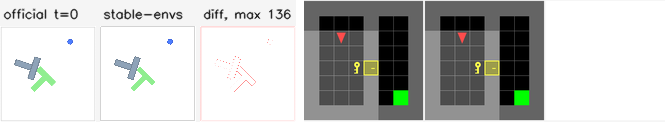
\includegraphics[width=0.8\columnwidth]{figures/parity.png}
\caption{Official renderer, ours, and the absolute difference, on identical
states. Left: PushT at 96\,px, where the residual is exactly the anti-aliased
outline and interior agreement is 100.00\%. Right: MiniGrid DoorKey, whose
difference column is empty --- the tile-atlas path is byte-exact.}
\label{fig:parity}
\end{figure}

\begin{table*}[t]
\centering
\caption{Fidelity: all \seNenvs{} environments, in the two tiers the registry
separates. Every number is against that environment's \emph{own} official
renderer on states from its own reset distribution; \emph{interior} pixels are
those whose $3\times3$ neighbourhood in the reference is one flat colour, and
Section~\ref{sec:fidelity} reports where that premise itself fails. The
\emph{visual} tier is not a weaker parity claim but a different one: it is
barred from claiming parity at all, declares an SSIM instead, and its test
asserts that SSIM. Throughput and storage are a separate claim
(Table~\ref{tab:family}).}
\label{tab:coverage}
\vskip 0.06in
\scriptsize
\setlength{\tabcolsep}{4pt}
\renewcommand{\arraystretch}{0.94}
\begin{tabular}{lrllll}
\toprule
Family & Envs & Reference & All pixels exact & Interior exact & Measured over \\
\midrule
% tier counts: 164 parity + 32 visual = 196; fidelity_tier / parity_interior_min=None across stable_envs/envs/
\multicolumn{6}{l}{\emph{Parity tier --- 164 environments. The interior claim is 1.0 unless a \texttt{parity\_note} names a mechanism.}}\\
\midrule
% parity: docs/research/classic_control.md sec.4 (0 of 250.9M px, 256/256 frames)
Classic control      & 5  & gymnasium 1.2.3          & \textbf{100.00000\%} (0 / 250.9\,M px) & \textbf{1.0} & 256 frames / env \\
% parity: docs/research/minigrid.md sec.5 (21,216 frames, max abs 0)
MiniGrid + BabyAI    & 7$^{\dagger}$ & minigrid 3.1.0 & \textbf{max $|\Delta| = 0$} & \textbf{1.0} & 21,216 frames \\
% parity: docs/research/pixel_native.md sec.5 (MiniHack, Craftax, Procgen), crafter.md, sokoban.md
Tile / sprite atlas  & 8  & 5 packages$^{\ddagger}$   & \textbf{100\%}, max $|\Delta| = 0$ & \textbf{1.0} & every enumerated tile \\
% parity: docs/research/griddly.md sec.1 (200 frames/game build gate, max abs 0)
Griddly              & 7  & griddly 1.6.7            & \textbf{100\%}, max $|\Delta| = 0$ & \textbf{1.0} & 1,400 frames \\
% parity: docs/research/overcooked.md sec.1 line 24 (JaxMARL visualizer, max abs 0)
Overcooked           & 5  & jaxmarl 0.1.0            & \textbf{100\%}, max $|\Delta| = 0$ & \textbf{1.0} & 64 states / env \\
% parity: docs/research/jumanji.md "Parity against the official renderer" (8 envs, mean 0.0000/255)
Jumanji              & 8  & jumanji 1.1.2            & \textbf{100\%}, max $|\Delta| = 0$ & \textbf{1.0} & 512 states \\
% parity: docs/research/pgx.md "The result"; stable_envs/envs/pgx.py:509
PGX board games      & 4  & pgx / resvg              & 91.5--98.4\% & \textbf{1.0} & 16 states / env \\
% parity: docs/testing.md (96px ss=1/ss=2: interior 100.00%, all 90.70/93.79%)
PushT                & 1  & gym\_pusht               & 90.7--93.8\%$^{\S}$ & \textbf{1.0} & 96 and 224\,px \\
% parity: docs/research/highway.md sec.1 (interior 100%, all 99.933-99.997%)
highway-env          & 6  & highway-env 1.12.1       & 99.933--99.997\% & \textbf{1.0} & 6 scenarios \\
% parity: docs/research/lunarlander.md sec.2 and docs/research/carracing.md (CarRacing exact_frac 1.0)
Box2D (LunarL., CarRac.) & 2 & gymnasium + Box2D 2.3.10 & 99.969\% / \textbf{100\%} & \textbf{1.0} & 404 polygons (CarRac.) \\
% parity: docs/research/swm_coverage.md; floor: stable_envs/envs/swm_nav.py:356
2-D navigation       & 5  & stable\_worldmodel       & 99.94--99.9994\% & 0.9999991$^{\P}$ & 800 seeded draws \\
% parity: docs/research/ogbench.md "Packaged" (25 cells x 64 states, interior 1.000000)
OGBench mazes        & 25 & ogbench / MuJoCo         & 99.69--99.98\% & \textbf{1.000000} & 25 cells $\times$ 64 states \\
% parity: docs/research/maze2d.md (99.49-99.77%, interior 1.000000)
D4RL maze2d          & 4  & gym-robotics 1.4.2       & 99.49--99.77\% & \textbf{1.000000} & 64 states / env \\
% parity: docs/research/dmcontrol.md sec.6 (11 parity cells; all-pixel 0.90684-0.99824)
DM Control           & 11 & dm\_control 1.0.44       & 90.7--99.8\% & \textbf{1.000000}$^{**}$ & 64 states $\times$ 3 draws \\
% parity: docs/research/mujoco_locomotion.md sec.3; stable_envs/envs/mujoco_locomotion.py PARITY
Gymnasium MuJoCo     & 4$^{\|}$ & gymnasium 1.2.3    & 96.9--99.7\% & 0.99999--\textbf{1.0}$^{\|}$ & 41--101 seeded draws \\
% parity: docs/research/fetch.md sec.1; post-fix value logs/.../perf/fd_fin_627446.log
Fetch                & 12 & gym-robotics             & 90.8--92.8\% & 0.9988$^{\dagger\dagger}$ & 64 states $\times$ 12 ids \\
% parity: docs/research/metaworld.md sec.7; stable_envs/envs/metaworld.py:901
Meta-World           & 50 & metaworld 3.1.1          & 81.5--88.4\% & 0.9997 med.$^{\ddagger\ddagger}$ & 64 states $\times$ 50 tasks \\
\midrule
\multicolumn{6}{l}{\emph{Visual tier --- 32 environments, which may not claim parity. The asserted quantity is SSIM; interior exactness is reported and never asserted.}}\\
\midrule
% source: stable_envs/envs/mujoco_locomotion.py VISUAL_FIDELITY; docs/research/mujoco_locomotion.md sec.7.1
MuJoCo locomotion    & 6  & gymnasium / nvdiffrast   & SSIM 0.947--0.981 & 0.54--0.88 & 64 states $\times$ 4 draws \\
% source: stable_envs/envs/dmcontrol.py VISUAL_FIDELITY; docs/research/dmcontrol.md sec.8
DM Control (track)   & 5  & dm\_control / MJWarp     & SSIM 0.661--0.964 & 0.0002--0.649 & 64 states $\times$ 3 draws \\
% source: stable_envs/envs/humanoidbench.py FIDELITY; docs/research/humanoidbench.md
HumanoidBench        & 17 & humanoid\_bench 0.2      & SSIM 0.849--0.931 & 0.607--0.943 & 64 states $\times$ 4 draws \\
% source: stable_envs/envs/robocasa.py FIDELITY; docs/research/robocasa.md sec.17.2
RoboCasa             & 4  & robocasa 1.0.1 / MJWarp  & SSIM 0.821--0.921 & 0.048--0.158 & 64 states $\times$ 4 draws \\
\bottomrule
\end{tabular}
\vskip 0.04in
{\scriptsize $^{\dagger}$~plus 165 further ids on demand; the offline
validation covers all 172 instantiable ones. $^{\ddagger}$~\texttt{nle},
\texttt{craftax}, \texttt{crafter}, \texttt{gym-sokoban}, \texttt{procgen}
(4 games). $^{\S}$~at 96\,px, supersample 1 and 2; the residual is
anti-aliasing (Figure~\ref{fig:parity}); at 224\,px interior parity is
99.9985\%. $^{\P}$~the worst of 800 seeded draws; the floor is declared at 0.999995 and
its mechanism is one ulp of float32 \texttt{exp} and not geometry --- 2 pixels
of 2.3\,M, at 1/255, on one channel (Section~\ref{sec:fidelity}).
$^{**}$~1.0 on the seven cells where the metric is defined; on the other four
a DM Control frame has no flat $3\times3$ neighbourhood at all and the suite
falls back to all-pixel agreement, where \texttt{finger-turn\_easy} declares
0.89. $^{\|}$~4 of gymnasium's 10, the other 6 being the visual-tier row
below; 1.0 on \texttt{Reacher} and \texttt{InvertedDoublePendulum} (0 of 41
seeded draws below), 0.99999 declared on \texttt{InvertedPendulum} and on
\texttt{Pusher}, whose 1.0 turned out to be one lucky draw
(Section~\ref{sec:fidelity}). $^{\dagger\dagger}$~measured; the floor is declared at 0.99 with a
\texttt{parity\_note}. 91\% of the frame is a plate baked through MuJoCo at
interior-exact 1.0, and 98.3\% of the interior residual is the arm's 18 STL
meshes, which MuJoCo
Gouraud-interpolates and this renderer shades per pixel (interior mean
$|\Delta|$ 0.009/255). It reads 0.9988 rather than 0.9923 because of the
CUDA-graph fix in Section~\ref{sec:fidelity}. $^{\ddagger\ddagger}$~median over 3,200 frames;
minimum 0.9808, floor declared at 0.978, and 48 of 50 tasks are above 0.99. The all-pixel column is low because the Sawyer arm covers 12.5--16.7\%
of the frame, not because the renderer is worse.}
\end{table*}

\section{Coverage, fidelity and throughput}
\label{sec:coverage}

\textbf{Interior pixels are the strong claim, and most --- not all --- are held to 1.0.} An
interior pixel has no coverage ambiguity, so a disagreement there is a wrong
colour, shape or place; all-pixel agreement is looser, because edges are two
anti-aliasing rules landing on different sides of a rounding and the reference
is not ground truth there. Folding the two together
is the failure mode: a mitred instead of round block outline costs 2.2\% of
PushT's interior pixels and is invisible in an all-pixel average. A lower floor
may be declared only with a \texttt{parity\_note} naming the mechanism, and
each of the four declaration sites names a specific arithmetic cause rather than
an effort budget --- Meta-World's Sawyer meshes, Fetch's 18 Gouraud-shaded
meshes, two MuJoCo locomotion cells, and 2-D navigation's one ulp of
\texttt{exp} (Section~\ref{sec:fidelity}).

\textbf{Those four sites cover 68 of the 159 parity-tier environments, and we
state that rather than the site count.} Meta-World alone is 50 at a floor of
0.978 and Fetch 12 at 0.99; the remaining floors are 0.99999 and 0.999995. So
``held to 1.0'' describes 91 environments exactly and 68 approximately, and the
gap is not cosmetic: a floor of 0.978 permits 2.2\% of interior pixels to
disagree, which is precisely the magnitude of the mitred-outline defect used
two sentences earlier as the canonical example of an error worth catching. The
defence of the floor is that its \emph{mechanism} is named and bounded, not
that its magnitude is negligible --- and a reader comparing families should
read Table~\ref{tab:coverage} per family rather than the tier label.
% source: scratch/census/counts.sbatch (159 parity / 68 below 1.0: metaworld 50, fetch 12,
% swm_nav 4, mujoco_locomotion 2; floors 0.978/0.99/0.99999/0.999995); docs/testing.md;
% stable_envs/envs/mujoco_locomotion.py PARITY; stable_envs/envs/fetch.py parity_interior_min; stable_envs/envs/swm_nav.py:356

\textbf{The throughput column is not one measurement, and saying so is the
correction this version makes.} Two mistakes were live in the previous
numbers, and both inflated them.

\emph{First, the resolution was not the one users get.} The sweep passed
\texttt{-{-}ss~1} while \seNssTwo{} registered classes declare
\texttt{default\_supersample = 2} --- the 25 OGBench mazes and the 4 D4RL
mazes --- because their
reference is MSAA'd and a hard silhouette is the wrong answer at a mover's
edge. Those rows
therefore described a picture four times cheaper in rays than the one
\texttt{se.make(name)} returns, and it is the same picture every parity number
in Table~\ref{tab:coverage} is measured on. The flag now defaults to
\texttt{native} and the affected rows were re-measured; the A/B on one process
and one idle node is 1.16--3.3$\times$, not the 4$\times$ the ray count would
predict, for the reason that follows.
% source: examples/bench_gpu_vs_cpu.py make_env docstring; examples/results/decode/ALL.json ss field (44 rows)

\emph{Second, most of these rows are host-bound, so their throughput is partly
a property of the node.} The previous claim that ``the GPU column reproduces
across nodes to 0.4\%'' was verified on the fused 2-D rasterizer at one
operating point and generalised to rows where it does not hold. Measuring
process CPU seconds per wall second inside the timed loop settles it: of
\seNhostRows{} rows, \seNhostAbove{} sit at or above 100\%, the median is
\seHostMedian\% and the worst is \seHostMax\% --- several cores saturated in a
per-chunk Python loop with the device waiting. The consequence is measurable
rather than theoretical: \texttt{DMCBallInCupCatch} at 84\,px, batch 4096,
gave \textbf{3,664 frames/s on an idle node and 271--978 on contended ones}, a
13$\times$ spread on a column that claimed 0.4\%. Every row now carries its
resolved supersample, its \texttt{cpu\_frac} and the load average, and a row
with \texttt{cpu\_frac} near or above 1 should be read as a measurement of the
host as much as of the device.
% source: examples/bench_gpu_vs_cpu.py module docstring; examples/results/decode/ALL.json cpu_frac; logs .../audit/dmcanat2_627223.log, ssfix2_dmc_627242.log

\textbf{Storage is the claim that does not depend on any of this.} Summed over
the registry the state that determines a frame is \seStorageStateB\,B against
\seStorageRawB\,B of raw pixels, a factor of \textbf{\seStorageRatio}; the
per-environment median is \seStorageMedian$\times$ and the best is
\seStorageMax$\times$. Against JPEG rather than raw pixels it is still
\seJpegRatio$\times$. No throughput result moves those numbers, and the
resolution and appearance are chosen at render time, which no frame corpus
offers. 18 of the \seNenvs{} also ship a batched GPU \texttt{step}, at 476.6\,M
env-steps/s against 8,100--488,000 on CPU. Renderer parity and simulator parity
are different claims and are never stated in the same words: PushT tracks
pymunk to a \emph{median} 0.68\,px and says so, while MiniGrid and Sokoban are
\emph{exactly} equal over the enumerated cross product (\textbf{10,752} and
\textbf{9,216 transitions, 0 mismatched}).
% source: examples/paper/tables/stats.json "storage" (from examples/results/decode/ALL.json); README.md rollout table; stable_envs/envs/minigrid.py Physics section; docs/research/sokoban.md sec.5; examples/results/rollout_with_policy.json (block_median_err 0.683)

\begin{table*}[t]
\centering
\caption{Throughput and storage, per family, at a single operating point ---
$256\times256$, batch 1024 --- so the rows compare environments rather than
operating points. \emph{State\,:\,frame} is bytes of state against raw bytes of
frame and is the storage claim; it does not depend on any timing.
$\times$\emph{default} is against the environment's own official renderer, one
frame at a time, which is the only entry point it offers.
$\times$\emph{stored} is against \textbf{the bar that decides the thesis}:
JPEG-in-Lance at quality 95, the layout \texttt{stable\_worldmodel} writes,
read a chunk of rows at a time and batch-decoded through libjpeg-turbo across
\textbf{eight worker processes} from node-local NVMe with the page cache warm
--- the fastest \emph{CPU} path measured. It is not the fastest path measured:
nvJPEG decoding on the GPU is, at \seGpuFps{} frames/s, and the table reports
that divisor beside it rather than in an appendix, because dividing by the
faster CPU path while a faster GPU path exists in the same document would be
choosing the conclusion. Against \emph{one} core the comparison would be
\seStoredWorkerFactor$\times$ kinder again (Appendix~\ref{app:storage-paths}). The rule separates the families that beat it from
the families that do not. Per-environment rows in
Appendix~\ref{app:throughput}. Sokoban is the one family of the
\seNfamilies{} with no stored row --- its frames were never written into the
Lance table --- so the ratio columns cover \seNfamRated{}. This table is
generated by \texttt{make\_tables.py}; no number in it is transcribed.}
\label{tab:family}
\vskip 0.06in
\footnotesize
\setlength{\tabcolsep}{4.2pt}
\renewcommand{\arraystretch}{0.95}
% GENERATED by examples/paper/make_tables.py -- do not edit by hand
\begin{tabular}{lrlrrrrr}
\toprule
Family & Envs & State\,:\,frame & Ours f/s & $\times$default & $\times$stored$_{\mathrm{cpu}}$ & $\times$stored$_{\mathrm{gpu}}$ & Range $\times$stored$_{\mathrm{cpu}}$ \\
\midrule
Griddly & 7 & 1/432 & 2,269,046 & 15,653$\times$ & \textbf{187$\times$} & 96$\times$ & 53--354 \\
Overcooked & 5 & 1/768 & 3,541,083 & 4,080$\times$ & \textbf{137$\times$} & 110$\times$ & 107--168 \\
MiniHack & 1 & 1/192 & 238,253 & ---$\times$ & \textbf{74$\times$} & 14$\times$ & --- \\
MiniGrid / BabyAI & 7 & 1/734--1/768 & 347,003 & 888$\times$ & \textbf{23$\times$} & 12$\times$ & 15.3--85.8 \\
Jumanji & 8 & 1/300--1/556 & 542,697 & 80,362$\times$ & \textbf{19$\times$} & 18$\times$ & 13.8--34.4 \\
Craftax & 1 & 1/95 & 521,291 & ---$\times$ & \textbf{13$\times$} & 20$\times$ & --- \\
PushT & 1 & 1/1,382 & 254,551 & 534$\times$ & \textbf{11$\times$} & 7.74$\times$ & --- \\
Procgen & 4 & 1/5--1/16 & 101,504 & 107$\times$ & \textbf{9.19$\times$} & 4.64$\times$ & 3.2--14.8 \\
PGX & 4 & 1/579--1/4,800 & 94,329 & 1,855$\times$ & \textbf{5.74$\times$} & 3.34$\times$ & 4.89--6.45 \\
highway-env & 6 & 1/1,406--1/30,000 & 70,761 & ---$\times$ & \textbf{4.94$\times$} & 2.54$\times$ & 3.9--11.1 \\
swm nav & 5 & 1/9,408--1/93,750 & 115,646 & 225$\times$ & \textbf{4.90$\times$} & 3.41$\times$ & 2.69--9.80 \\
OGBench & 25 & 1/1,344--1/18,816 & 78,569 & 183$\times$ & \textbf{4.51$\times$} & 2.44$\times$ & 2.5--10.8 \\
Crafter & 1 & 1/38 & 44,723 & ---$\times$ & \textbf{3.45$\times$} & 1.56$\times$ & --- \\
D4RL PointMaze & 4 & 1/9,408 & 65,103 & 32$\times$ & \textbf{3.42$\times$} & 2.15$\times$ & 3.20--3.65 \\
classic control & 5 & 1/90,000--1/180,000 & 14,257 & 32$\times$ & \textbf{2.38$\times$} & 0.55$\times$ & 1.81--3.33 \\
LunarLander & 1 & 1/4,737 & 11,583 & 34$\times$ & \textbf{1.91$\times$} & 0.44$\times$ & --- \\
DM Control & 16 & 1/189--1/5,292 & 22,819 & 64$\times$ & \textbf{1.45$\times$} & 0.75$\times$ & 0.25--5.36 \\
Fetch & 12 & 1/6,912--1/9,600 & 20,799 & 32$\times$ & \textbf{1.08$\times$} & 0.66$\times$ & 1.06--1.13 \\
\midrule
HumanoidBench & 17 & 1/592--1/1,890 & 13,370 & 324$\times$ & \textbf{0.64$\times$} & 0.42$\times$ & 0.53--0.92 \\
MuJoCo locomotion & 10 & 1/1,800--1/21,600 & 9,422 & 25$\times$ & \textbf{0.56$\times$} & 0.32$\times$ & 0.51--2.18 \\
Meta-World & 50 & 1/7,513--1/14,400 & 7,179 & 34$\times$ & \textbf{0.45$\times$} & 0.25$\times$ & 0.20--0.49 \\
RoboCasa & 4 & 1/1,117--1/3,781 & 5,877 & 14$\times$ & \textbf{0.37$\times$} & 0.21$\times$ & 0.36--0.71 \\
CarRacing & 1 & 1/247 & 22,206 & 168$\times$ & \textbf{0.30$\times$} & 0.61$\times$ & --- \\
\bottomrule
\end{tabular}


\textbf{Against nvJPEG the speed claim is a wash, and we state it as one.} The
median environment is \seGpuMedian$\times$ and the geometric mean
\seGpuGeomean$\times$; \seNbelowGpu{} of \seNratedGpu{} environments are slower
than reading. That is the honest headline for the \emph{speed} half. It leaves
the thesis where it belongs: a faster decoder does not remove the frames from
disk, so the \emph{storage} claim --- \seStorageRatio$\times$ against raw pixels
and \seJpegRatio$\times$ against their JPEGs --- holds against every path in
this table, as does the configuration claim of
Section~\ref{sec:configuration}, and neither depends on which decoder a reader
happens to own.

\end{table*}

\section{Four findings about the tools}
\label{sec:fidelity}

Fusing the ray-cast path into one kernel was a throughput change that turned
into a fidelity investigation, and what it found is not specific to this
repository: it is true of Triton, of \texttt{mujoco\_warp}, and of the
interior-pixel metric that parity suites like this one are built on. Each was
found by a conformance check rather than by inspection, and each is stated here
with the flag or the fix that closes it.

\textbf{1. Triton's default \texttt{fp32} lowering is not bit-identical to
torch, and three flags close it.} Over 4.2\,M random inputs per shape, a fused
kernel disagrees with the same arithmetic in torch on 836,950 patterns for
$ab+c$, 1,492,420 for a 3-vector dot product, 1,249,701 for $a/b$ and 709,903
for $\sqrt{\vphantom{b}a}$. \texttt{enable\_fp\_fusion=False} on the first two,
\texttt{tl.math.div\_rn} on the third and \texttt{tl.sqrt\_rn} on the fourth
take all four to \textbf{exactly zero}. The residue is that
\texttt{torch.pow} against libdevice \texttt{powf} does \emph{not} close ---
1.5--1.7\,M of 4.2\,M still differ, at 1 ulp --- which is why shading stayed
outside the fused kernel rather than being made approximately equal inside it.
\texttt{torch.compile} is not a substitute for the flags: Inductor emits fused
Triton with floating-point fusion \emph{on}, so compiling a reference
implementation changes its output.
% source: logs .../perf/tri2_627128.log (four shapes, both settings); .../perf/pow_627579.log (libdevice.pow)

The same suite had already found the matching bug one level up:
\emph{\texttt{torch.einsum} is not batch-size reproducible}, because it lowers
to \texttt{bmm} and cuBLAS picks the kernel --- and with it the summation
order --- from the gemm \emph{count}. One ulp then enters the ray quadratic as
$\mathrm{disc} = b^2 - ac$, a difference of nearly equal numbers on a
silhouette ray, which amplified it ${\sim}10^{4}\times$ into a hit/miss flip:
8--44 pixels a frame, up to 59/255, on 17 of the 25 OGBench cells. A renderer
held to bit-exactness cannot treat either of these as a tuning detail.
% source: stable_envs/render/raycast3d.py frame-changes comment; docs/research/ogbench.md

\textbf{2. A CUDA graph can capture the wrong kernel, and nothing reports it.}
\texttt{mujoco\_warp.render} defines its megakernel \emph{inside} the call, so
the kernel's source is regenerated per call from whatever quantiser is bound at
that moment. A graph captured outside a \texttt{with gl\_rounding()} block
therefore replays the \emph{truncating} kernel for the rest of the run, while
every later call looks correct in isolation. The signature is unambiguous
because a quantisation swap can only be $\{0, -1\}$: against correct rounding
the captured graph differed on \textbf{15.8\% of Fetch interior channels,
21.2\% of Meta-World's and 63.8\% of HumanoidBench's}, and was bit-identical to
the truncating kernel. Capturing inside the block inverts both lines exactly,
and moves Fetch's interior parity \textbf{0.9923 $\to$ 0.9988}. The general
statement --- a graph freezes whichever kernel was live at capture, including
one selected by a context manager --- applies to any framework that generates
kernels at call time.
% source: scratch/perf/rounding.py docstring; logs .../perf/rd_ft_627149.log, rd_mw_627150.log, rd_hb_627151.log; fd_leg_627187.log vs fd_fin_627446.log

\textbf{3. The interior-pixel metric is sound for flat-shaded rasterizers and
unsound for smooth ones, and we can say exactly where it breaks.} ``Flat
$3\times3$ in the reference'' is a proxy for ``no rounding ambiguity here'',
and that implication holds only when the renderer fills flat-coloured
primitives. The 2-D navigation family is the counterexample, and its residual
decomposes completely: run on CPU with the reference's own float32
\texttt{exp}, our renderer is bit-for-bit identical to the official one, and
the device contributes nothing. What is left is that torch's \texttt{exp} is
1-ulp \emph{faithful} while ours is \emph{correctly rounded}, and the ulp flips
a pixel only where a shaded colour lands exactly on the background value --- in
the middle of a flat region, which is precisely where the metric promises there
is nothing to decide. It is now a declared floor of 0.999995 with a
\texttt{parity\_note}: worst of 800 seeded draws, 2 pixels of 2.3\,M, 1/255,
one channel.

Seeding the parity tests to write that floor exposed a second one. MuJoCo's
Pusher declared an interior floor of 1.0 on the strength of a \emph{single
unseeded draw}; run over 101 independent draws it fails \textbf{15 of them}, at
1--2 pixels of 3.03\,M. The other 86 are exact, and the original draw was one
of those. Two controls in the same family do not move at all --- Reacher and the
inverted double pendulum, 0 of 41 draws each --- which is what says this is the
environment and not the harness. \emph{An unseeded parity test does not measure
a floor; it samples one.}
% source: stable_envs/envs/swm_nav.py:356; logs .../audit/swmmech3_627119.log; scratch/audit/pusher_parity_rate.py; logs .../audit/mjlocrate_627330.log (15/101), mjlocrate2/3 (0/41)

\textbf{4. In \texttt{mujoco\_warp}, a frame depends on which world slot drew
it.} HumanoidBench's long-standing non-determinism under batching reduces to
this: the library builds \emph{one} BVH over all
$\mathrm{nworld} \times \mathrm{ngeom}$ primitives at once, so identical
geometry placed in different slots gets differently shaped subtrees, and
closest-hit ties break by visit order. Filling all 64 worlds with the
\emph{same} \texttt{qpos} and comparing against slot 0 isolates it with
nothing else varying: H1-balance-simple differs on 2 pixels at 1/255, in slots
21 and 42, and eight sibling cells differ on none. The same cause explains the
larger chunk-size effect (1--13 pixels at up to 128/255, non-monotone in world
count). The fix is a deterministic tie-break at equal ray parameter and it
belongs upstream, not here; until then the affected cells are in the visual
tier, where the asserted quantity is an SSIM that this does not move.
% source: scratch/perf/worldslot.py; logs .../perf/ws_hb_627394.log, ci_hbn_627370.log; docs/research/humanoidbench.md

\section{The configuration is the contribution}
\label{sec:configuration}

The throughput argument is the one a reader expects and the one we lose against
the strongest decoder (Section~\ref{sec:coverage}). It is also not the reason to
do this. The reason is that \textbf{a stored corpus fixes, at collection time,
every choice the experiment has not been designed yet to make}: the camera pose,
the resolution, the palette, whether the goal is drawn, whether the walls are
visible. Those are exactly the variables a study varies.

\textbf{Stored frames multiply; states do not.} An ablation over $R$ resolutions
and $A$ appearances needs $R\!\times\!A$ corpora --- each generated, named,
versioned, and kept mutually consistent, with the provenance of every one
tracked well enough that a reviewer can tell which produced which figure. Adding
a third axis multiplies again. The state corpus is written \emph{once}; $R$ and
$A$ become arguments to \texttt{render}, and the artefact that has to be
archived for reproducibility is the state file plus a config, not the cross
product. This is the difference between an ablation that costs a re-collection
and one that costs a loop.

\textbf{And the cross product is free at batch scale, because appearance is a
tensor rather than a re-render.} Every variation leaf lands in a per-world field
of one kernel launch, so a batch of distinct appearances costs one launch rather
than $B$. On PushT (29 appearance dimensions) one batch produces \textbf{1,024
distinct appearances in 2.85\,ms}, \textbf{715$\times$} faster than looping the
same renderer over the same 1,024 styles, and 4,096 in 4.09\,ms
(\textbf{1,986$\times$}, 1.00\,M frames/s).
% source: examples/results/domain_randomization.json rows[]; style_dim 29; grid distinct 64/64
Every frame is verified distinct rather than assumed to be: the 64-cell grid
reports \textbf{64/64} distinct, which is what separates a working randomisation
from a knob that silently collapsed to environment~0.

\textbf{The defaults are the official appearance, so this costs nothing to
ignore.} A variation space whose zero point is a stylisation would make every
parity number in this paper a claim about our taste; instead the declared
default reproduces the reference renderer bit for bit
(Table~\ref{tab:coverage}), and randomisation is opt-in on top of a frame that
is already exact.

\textbf{What this does not give you.} The axes are the ones an environment
\emph{declares}; a camera the reference renderer cannot express is not
reachable, and for the visual tier the appearance knobs move a frame that was
already a different render (Section~\ref{sec:nogo}). Nor does it help if the
corpus you have is frames: recovering states from pixels is not part of this
work, and the one-time cost of re-running rollouts to record states is real and
is the main adoption barrier we observe.

\section{Does it substitute?}
\label{sec:substitute}

Pixel parity is a claim about bytes; the claim that matters is about
consequences. The strongest available test is to take an official pretrained
model, run \emph{its own} evaluation unchanged, and swap only the pixels it
sees. We use the LeWorldModel PushT checkpoint --- a ViT world model trained
end to end on frames from the official pygame renderer --- with its own
\texttt{eval.py}, config, dataset and CEM planner. The arms are
\emph{paired}: for each seed the episode indices, start steps, goal offset and
CEM seed are identical, so episode $i$ is the same task in both. Over six
seeds $\times$ 50 episodes the gap is $-0.3$ points, against a seed-to-seed
spread of 80--96\% in the official arm.

\textbf{The control is what makes the null mean something.} Success is computed
from the pymunk state and never reads a pixel, so an unchanged score is
evidence only if the score \emph{can} change. Blank frames cost 92 points and
flip 46 of 50 episodes at $p < 0.001$, while replacing only the ${\sim}1{,}487$
live observations per run leaves the success count \emph{exactly} where it was.
% source: examples/lewm_pusht/results/summary.txt; examples/lewm_pusht/README.md

\textbf{The stored corpus is a degraded copy of the renderer's output.} The
only arm that moves at all is the one replacing the two \emph{stored} corpus
frames per run, and diagnosing it inverts the usual objection to regeneration.
At 224\,px over 48 corpus states our raster matches the live official
renderer on \textbf{100.00\%} of interior pixels, while the corpus's own stored
frames match it on 91.9\%, carrying \textbf{1,582 distinct colours each}
against 146 for the live pygame path and \textbf{7} for a flat-shaded raster
--- the entire palette --- and nine resize filters and eight round trips fail
to reproduce it, every one coming out \emph{sharper}. Those 46.3\,GB are a
lossy copy: regenerating from the states is strictly \emph{closer} to the
reference than reading them off disk.
% source: examples/lewm_pusht/results/parity_224.json (ours_direct interior_exact_frac 1.0; stored 0.9191)

\begin{table}[t]
\centering
\caption{A pretrained PushT world model cannot tell our frames from the
official ones, while the same evaluation detects a broken renderer at
$p < 0.001$. Paired McNemar exact test; ``disc.'' counts discordant pairs.}
\label{tab:lewm}
\vskip 0.06in
\footnotesize
\setlength{\tabcolsep}{3.5pt}
\begin{tabular}{lrrl}
\toprule
Frames the model sees & Succ. & SR & Paired vs official \\
\midrule
% source: examples/lewm_pusht/results/summary.txt
official (pygame)        & 264/300 & 88.0\% & --- \\
stable-envs, every px    & 263/300 & \textbf{87.7\%} & 12/11 disc., $p = 1.000$ \\
\quad live obs.\ only    & 264/300 & 88.0\% & \phantom{0}2/2 disc., $p = 1.000$ \\
\quad corpus frames only & 259/300 & 86.3\% & 17/12 disc., $p = 0.458$ \\
blank frames (control)   & \phantom{00}2/50 & 4.0\% & 46/0 disc., $\mathbf{p < 0.001}$ \\
\bottomrule
\end{tabular}
\end{table}

\begin{table*}[t]
\centering
\caption{The criterion applied. The verdict column now has three values rather
than two, because measurement forced a middle one: a family can clear G1--G3
and still not pay on G4, in which case it ships with the claim it can support
and the shortfall printed (Table~\ref{tab:family}) rather than being dropped or
oversold.}
\label{tab:gates}
\vskip 0.06in
\scriptsize
\setlength{\tabcolsep}{4pt}
\renewcommand{\arraystretch}{0.94}
\begin{tabular}{L{0.115\textwidth}L{0.185\textwidth}L{0.125\textwidth}L{0.175\textwidth}L{0.165\textwidth}L{0.10\textwidth}}
\toprule
Family & G1 purity & G2 state / frame & G3 decoder & G4 economics & Verdict (gate) \\
\midrule
% source: Table 1 (parity tier); tables/family.tex for the G2 and G4 ranges
Parity tier, 164 envs & exact (Table~\ref{tab:coverage}) & 1/5--1/\seStorageMax & atlas, $\le 19$ analytic primitives, or a baked plate; family-wide & mostly yes: \seNfamAbove{} of \seNfamRated{} families beat the stored path, to \seStoredMax$\times$ (Table~\ref{tab:family}) & \textbf{GO} (shipped) \\
% source: docs/research/metaworld.md sec.1 (probe_state_gate.py rungs R0-R4), sec.7
Meta-World, 50/50 & \emph{withdrawn}: a reset writes placement into the \emph{model}, but restoring 14 model arrays makes a different episode bit-exact on \textbf{50/50} (control: 0/50) & \texttt{qpos} + 0--6 named floats & \emph{withdrawn}: ported and measured, interior median \textbf{0.9997} & no (Table~\ref{tab:family}) & \textbf{GO} at parity, \textbf{loses G4} \\
% source: Table 1 visual tier; docs/research/robocasa.md sec.10, 11; humanoidbench.md
Visual tier, 32 envs & yes & 1/189--1/21,600 & partly: \texttt{track} rides the body (MuJoCo loco., DM Control); \texttt{ngeom} 1,201--2,341 per reset (RoboCasa) & no (Table~\ref{tab:family}) & \textbf{SSIM only}; parity barred, \textbf{loses G4} \\
% source: docs/research/robocasa.md sec.9, 10, 11, 15
RoboCasa, at parity & exact, but only for a fixed compiled model & 1/135 per step; \texttt{ep\_meta} is 1.7\,kB gzipped and replays \textbf{99.6\%} & no: \texttt{ngeom} 1,201--2,341 per reset, 24\,GB of assets & no: exact $=0.37$ cores of decode; fast $=3.2$--$5.1$ at 0.06--0.23 interior-exact & NO-GO (\textbf{G4}) \\
% source: docs/research/pixel_native.md sec.1
Atari / ALE & no: identical 128\,B RAM differs on 13.75\% of pairs & \emph{passes}: $0.43\times$ & no: per-ROM 6507 + TIA emulator, no atlas & moot: 6.6k--54k fps per core & NO-GO (\textbf{G1, G3}) \\
\bottomrule
\end{tabular}
\end{table*}

\subsection{What a frozen encoder sees, on every family}
\label{sec:dino}

Table~\ref{tab:lewm} answers the consequence question hard for one environment
and one checkpoint. This is the cheap, wide complement: freeze
\seDinoModel{}, embed both renders of the \emph{same} state, and measure the
cosine distance across every family whose reference renderer is installed
(\seDinoN{} states each). \textbf{The controls are the measurement.} A distance
of 0.01 means nothing alone --- a metric that cannot move is small for a broken
renderer too --- so each environment is also measured against a JPEG q95
round-trip of the official frame (what a stored corpus would actually have
held), against two \emph{different} states through the same renderer (the scale
of a real difference), and against a blank frame (the broken floor).

\begin{table}[t]
\centering
\caption{Median cosine distance in \seDinoModel{} feature space, by fidelity
tier. \emph{Ours} and \emph{JPEG q95} are two ways of not being the official
frame; \emph{2 states} is what a genuinely different state costs; \emph{blank}
is the floor. Split by tier and never pooled: the visual tier is a different
render of the same scene by construction, so a pooled mean would flatter it and
slander the parity tier at once.}
\label{tab:dino}
\vskip 0.06in
\footnotesize
% GENERATED by examples/paper/make_tables.py -- do not edit by hand
\begin{tabular}{lrrrrr}
\toprule
Tier & Envs & Ours & JPEG q95 & 2 states & Blank \\
\midrule
parity & 159 & \textbf{0.0135} & 0.0131 & 0.0222 & 0.865 \\
visual & 33 & \textbf{0.0997} & 0.0076 & 0.2302 & 0.945 \\
\bottomrule
\end{tabular}

\end{table}

\textbf{On the parity tier we are level with JPEG, not ahead of it.} Ours is
\seDinoParityOurs{} against JPEG's \seDinoParityJpeg{} over
\seDinoParityN{} environments, and ours is the closer of the two on
\seDinoParityCloser{} of them --- a little over half. The residual is the
anti-aliased silhouette that the interior mask deliberately excludes, so it is
consistent with the interior-exact medians of 1.0 in Table~\ref{tab:coverage};
it is not consistent with a claim that the frames are interchangeable to a
model. \textbf{And it is not negligible against the right yardstick}: at
\seDinoParityPctScale\% of the distance between two different states, this is
the quantity a world model discriminates on. The honest statement is that the
difference is far below a destroyed frame (\seDinoParityBlank{}) and comparable
to the loss already accepted by storing JPEGs --- not that a model cannot see
it.

\textbf{On the visual tier the encoder separates the two easily, which is the
tier's own claim showing up in a measurement.} Ours is \seDinoVisualOurs{}
against JPEG's \seDinoVisualJpeg{}, and ours is closer on
\seDinoVisualCloser{} of \seDinoVisualN{} environments. That is the expected
sign: a visual-tier environment never asserted the same picture, only a
declared SSIM and mean-absolute band (Section~\ref{sec:fidelity}). It does mean
a frozen encoder is a \emph{sharper} instrument than the pixel metrics these
environments are held to, and anyone substituting visual-tier frames into a
pretrained pipeline should measure rather than assume.

% source: examples/results/dino/dino_agreement.json; examples/dino_agreement.py

\section{When it does not}
\label{sec:nogo}

A list of successes is not a result; the useful artefact is a rule that says in
advance where the approach helps and can say no. It pays when the frame is a
lookup into a decoder that is a \emph{constant of the family}, indexed by a
small per-step state; it fails when the decoder is itself content, regenerated
per episode (RoboCasa, \citealt{robocasa}) or written per title (Atari,
\citealt{ale}). Operationally that is four gates, each at most an afternoon. \textbf{G3, decoder stability}: reset twice and compare the compiled
scene, atlas or primitive set. \textbf{G1, purity}: drive two different
internal states to the same candidate state and demand \emph{0} differing
pixels. Purity can also hold only on a \emph{restricted} state space, and that
restriction is part of the claim rather than a footnote to it: Crafter reaches 0
differing pixels on 512/512 states \emph{provided} \texttt{daylight}~$\ge 0.5$,
because below that its reference draws noise from \texttt{world.random} and the
frame is not a function of any state at all. The env ships with the narrowed
space; a family whose purity needed a restriction nobody could state would fail
this gate.
% source: docs/research/crafter.md sec.G1 \textbf{G2, compression}: the render-relevant \emph{slice} of the state
over frame bytes must be below 1 --- the qualifier is the gate, since Craftax
and Crafter both ship a state larger than their frame and are wins on the
window drawn. \textbf{G4, economics}: regeneration must beat decoding a stored
frame \emph{at the fidelity the family requires}. A criterion that only ever
predicts success is not a criterion, and Table~\ref{tab:gates} contains both
outcomes --- plus a third that this round of measurement forced into existence.
% source: docs/research/pixel_native.md sec.3, docs/research/crafter.md

\textbf{G4 failing does not have to mean not shipping, and pretending it did
was the previous version's mistake.} The \seNfamBelow{} families below the rule
in Table~\ref{tab:family} clear G1--G3 and reach a declared fidelity, and still
lose to reading. Dropping them would hide a measurement; shipping them without
the ratio would oversell one. They ship with the ratio printed, and with the
observation that the \emph{storage} argument is untouched --- a Meta-World frame
is still 1/7,513 to 1/14,400 of its state --- which is why a state corpus is
still the right artefact for them even where a GPU is not the fastest way to
read one back.
% source: tables/family.tex (the rows below the rule); Meta-World state:frame from the same table

\textbf{RoboCasa remains the sharpest boundary, and it is a boundary about
\emph{fidelity}, not about kitchens.} A parity claim requires 100\% of interior
pixels, and only MuJoCo's own renderer can meet that for a kitchen, because it
\emph{is} the official one. Compiled, resident and stripped to what it draws
(verified bit-identical first), it saturates at \textbf{1,925 frames/s across
16 processes} at 128\,px against \textbf{5,137 for one CPU core of JPEG
decode}: 0.37 of a core. The fast alternative, MJWarp at 26,400 f/s, replaces
3.2--5.1 cores at \textbf{0.059--0.231} interior-exact. \emph{Exact costs
$2.7\times$ more than reading; fast is $4$--$17\times$ short of the parity
bar.} Both hold at $K = \infty$, so the failure does not depend on how a corpus
is bucketed. What ships is therefore the visual tier, at SSIM 0.821--0.921,
which is a claim the fast renderer can support and the parity tier is not.
% source: docs/research/robocasa.md sec.10, 11, 9; stable_envs/envs/robocasa.py FIDELITY

\textbf{Three rejections did not survive being measured, which is the other
half of the criterion working.} \textbf{Meta-World} \citep{metaworld} was a
NO-GO on G1 and G3: a reset writes the episode's placement into the
\emph{model}, so the frame is not a function of \texttt{qpos}. The conclusion
was wrong even though the observation was right. A ladder of progressively
larger restores locates what is missing exactly --- restoring
\texttt{qpos}/\texttt{qvel}/\texttt{ctrl}/\texttt{mocap} alone makes a
different episode bit-exact on 5 of 50 tasks, adding 14 model arrays makes it
\textbf{50 of 50}, and the control with nothing restored is \textbf{0 of 50} at
a median difference of 239/255. The render-relevant slice is 0--6 named floats
per task, so G2 is not endangered by widening the state, and all 50 now ship in
the parity tier. \textbf{CarRacing} was a NO-GO on four grounds, all of them
effort estimates; the real obstacle, found only by looking, is that the
environment draws through \emph{two} rasterizers in one frame ---
\texttt{gfxdraw.filled\_polygon} for the road and \texttt{pygame.draw.polygon}
for the car --- which agree on \textbf{14 of 404} polygons at identical integer
vertices, because the second rounds each row's crossings by the parity of how
many earlier-indexed edges are active, so the rule flips mid-edge. Transcribed,
it is exact. \textbf{DM Control} was blocked only by a version skew, and now
contributes 11 parity cells and 5 visual ones. \emph{Every rejection this
criterion has produced from an effort estimate rather than a measurement has
been overturned.}
% source: docs/research/metaworld.md sec.1 (probe_state_gate.py R0-R4); carracing.md blockers 1-5; dmcontrol.md sec.1

\textbf{The direction of the surprises is what makes this predictive.} The
families that look hardest are not the ones that fail: OGBench's articulated
humanoid reduces to 19 analytic primitives with \texttt{nmesh}~$=0$ and
NetHack's 1.27\,MB frame is a single gather, while Atari, the visually simplest
family, \emph{passes} the compression gate at $0.43\times$ and still fails on
purity and decoder. \textbf{Visual complexity is not the axis;
decoder stability is} --- and what decoder stability buys is the \emph{parity}
tier, which is a different question from whether the GPU is the fastest way to
get the pixels.

\section{Related work}

\textbf{GPU simulators.} Brax \citep{brax}, MuJoCo/MJX \citep{mujoco}, Isaac
Gym \citep{isaacgym}, Madrona \citep{madrona}, Craftax \citep{craftax}, Jax2D
\citep{kinetix}, EnvPool \citep{envpool} and CuLE \citep{cule} make simulation
fast, and several render on the GPU, but their fidelity claim is about their
own dynamics: they define a new fast environment, and results from one are not
comparable pixel-for-pixel with results from the environment it resembles. The
commitment here is the opposite --- parity against the \emph{official} renderer
of an environment the field already publishes numbers on --- and that
commitment is what forces the negative results.

\textbf{Compression and generation.} Distillation and condensation
\citep{distill,condense} shrink a corpus by learning a synthetic surrogate,
approximate and task-specific; here the compressor is the environment's own
renderer and the reconstruction is bit- or interior-exact. The families covered
are gymnasium and gymnasium-robotics \citep{gymnasium,gymrobotics},
MiniGrid/BabyAI \citep{minigrid,babyai}, MiniHack/NLE \citep{minihack,nle},
Craftax and Crafter \citep{craftax,crafter}, Sokoban \citep{sokoban}, OGBench
\citep{ogbench}, D4RL \citep{d4rl}, DM Control \citep{dmcontrol}, highway-env
\citep{highwayenv}, Procgen \citep{procgen} and PushT \citep{ibc,dp};
pixel-based world models \citep{worldmodels,dreamer,dinowm} are the consumer.

\section{Limitations and conclusion}

\seNfamBelow{} of \seNfamRated{} families do not beat the read path they are
meant to replace; Table~\ref{tab:family} says which, and the rule in it will
move again. The throughput of the ray-cast families is host-bound and therefore
a property of the node, so those ratios should be read as an order of
magnitude; the fix is to move the per-chunk loop off Python, and it is not
done. The
storage comparison is against warm node-local NVMe, which favours the stored
side; the shared filesystem a cluster corpus actually lives on is in
Appendix~\ref{app:storage-paths}. 178 of the \seNenvs{} environments ship no
simulator, by design, and no single interpreter holds the whole registry --- the
census spans 15 of them, and the widest single one reaches 147 --- because DM
Control needs \texttt{mujoco}~3.11 with \texttt{dm\_control}~1.0.44 while
OGBench's parity is calibrated against \texttt{mujoco}~3.9. Three families were rejected on our
judgement rather than by the criterion, which is a different list from the three
overturned above. Adroit clears G1--G3 under its fixed camera
and is still not buildable, because \texttt{mujoco\_warp} has no alpha path and
derives texture UVs for planes and meshes only. Franka Kitchen's Gate~1 was
closed on re-measurement, and its NO-GO now rests entirely on a plate argument
--- four casting lights over 85.6\% of the frame --- rather than on a gate.
And MiniWorld, whose camera \emph{is} the state, so there is no static plate to
bake: the argument usually given is that mipmap selection and Gouraud
interpolation over 29--66\% of the frame are implementation-defined, but the
stronger measured result is that \textbf{two conforming drivers} --- NVIDIA and
Mesa \texttt{llvmpipe}, given the identical scene, state and multisample count
--- agree on only \textbf{3.8--68.4\% of pixels (median 0.045)}. That is not a
port failing to match a reference; it is the same class of failure as Atari's,
where there is no single target to be exact against. That decoder is a vendor
binary.
% source: scratch/census/union.json (196 envs, 15 interpreters, widest 147); docs/research/dmcontrol.md sec.1; docs/research/adroit.md; docs/research/kitchen.md (Gate 1 closed 2026-08-10);
% docs/research/miniworld.md sec.G1 (NVIDIA vs Mesa llvmpipe, all-exact 0.0382-0.6839, median 0.0450)

The two halves of the thesis came apart under measurement, and that is the
result. An image corpus is redundant with a state corpus
\seStorageRatio$\times$ smaller for \emph{every} family here, regenerable at a
resolution and in a style chosen after the corpus was built, and no throughput
number touches that. Whether the GPU is also the fastest way to read it back is
a separate question with a per-family answer, and four cheap measurements say
which answer you get.

\begin{thebibliography}{99}
\raggedright
\setlength{\itemsep}{1pt}\setlength{\parsep}{0pt}
\providecommand{\natexlab}[1]{#1}

\bibitem[Bellemare et al.(2013)]{ale}
Bellemare, M.~G., Naddaf, Y., Veness, J., and Bowling, M.
\newblock The arcade learning environment: An evaluation platform for general
  agents.
\newblock \emph{Journal of Artificial Intelligence Research}, 47:253--279,
  2013.

\bibitem[Chevalier-Boisvert et al.(2019)]{babyai}
Chevalier-Boisvert, M., Bahdanau, D., Lahlou, S., Willems, L., Saharia, C.,
  Nguyen, T.~H., and Bengio, Y.
\newblock {BabyAI}: A platform to study the sample efficiency of grounded
  language learning.
\newblock In \emph{ICLR}, 2019.

\bibitem[Chevalier-Boisvert et al.(2023)]{minigrid}
Chevalier-Boisvert, M., Dai, B., Towers, M., de~Lazcano, R., Willems, L.,
  Lahlou, S., Pal, S., Castro, P.~S., and Terry, J.
\newblock Minigrid \& Miniworld: Modular \& customizable reinforcement learning
  environments for goal-oriented tasks.
\newblock In \emph{NeurIPS Datasets and Benchmarks}, 2023.

\bibitem[Chi et al.(2023)]{dp}
Chi, C., Feng, S., Du, Y., Xu, Z., Cousineau, E., Burchfiel, B., and Song, S.
\newblock Diffusion policy: Visuomotor policy learning via action diffusion.
\newblock In \emph{Robotics: Science and Systems}, 2023.

\bibitem[Cobbe et al.(2020)]{procgen}
Cobbe, K., Hesse, C., Hilton, J., and Schulman, J.
\newblock Leveraging procedural generation to benchmark reinforcement learning.
\newblock In \emph{ICML}, 2020.

\bibitem[Dalton et al.(2020)]{cule}
Dalton, S., Frosio, I., and Garland, M.
\newblock Accelerating reinforcement learning through {GPU} {A}tari emulation.
\newblock In \emph{NeurIPS}, 2020.

\bibitem[de Lazcano et al.(2024)]{gymrobotics}
de~Lazcano, R., Andreas, K., Tai, J.~J., Lee, S.~R., and Terry, J.
\newblock Gymnasium robotics.
\newblock \url{https://github.com/Farama-Foundation/Gymnasium-Robotics}, 2024.

\bibitem[Florence et al.(2021)]{ibc}
Florence, P., Lynch, C., Zeng, A., Ramirez, O., Wahid, A., Downs, L., Wong, A.,
  Lee, J., Mordatch, I., and Tompson, J.
\newblock Implicit behavioral cloning.
\newblock In \emph{Conference on Robot Learning}, 2021.

\bibitem[Freeman et al.(2021)]{brax}
Freeman, C.~D., Frey, E., Raichuk, A., Girgin, S., Mordatch, I., and Bachem, O.
\newblock Brax: A differentiable physics engine for large scale rigid body
  simulation.
\newblock In \emph{NeurIPS Datasets and Benchmarks}, 2021.

\bibitem[Fu et al.(2020)]{d4rl}
Fu, J., Kumar, A., Nachum, O., Tucker, G., and Levine, S.
\newblock {D4RL}: Datasets for deep data-driven reinforcement learning.
\newblock \emph{arXiv:2004.07219}, 2020.

\bibitem[Ha \& Schmidhuber(2018)]{worldmodels}
Ha, D. and Schmidhuber, J.
\newblock Recurrent world models facilitate policy evolution.
\newblock In \emph{NeurIPS}, 2018.

\bibitem[Hafner(2022)]{crafter}
Hafner, D.
\newblock Benchmarking the spectrum of agent capabilities.
\newblock In \emph{ICLR}, 2022.

\bibitem[Hafner et al.(2023)]{dreamer}
Hafner, D., Pasukonis, J., Ba, J., and Lillicrap, T.
\newblock Mastering diverse domains through world models.
\newblock \emph{arXiv:2301.04104}, 2023.

\bibitem[K\"uttler et al.(2020)]{nle}
K\"uttler, H., Nardelli, N., Miller, A.~H., Raileanu, R., Selvatici, M.,
  Grefenstette, E., and Rockt\"aschel, T.
\newblock The {N}et{H}ack learning environment.
\newblock In \emph{NeurIPS}, 2020.

\bibitem[Leurent(2018)]{highwayenv}
Leurent, E.
\newblock An environment for autonomous driving decision-making.
\newblock \url{https://github.com/Farama-Foundation/HighwayEnv}, 2018.

\bibitem[Makoviychuk et al.(2021)]{isaacgym}
Makoviychuk, V., Wawrzyniak, L., Guo, Y., Lu, M., Storey, K., Macklin, M.,
  Hoeller, D., Rudin, N., Allshire, A., Handa, A., and State, G.
\newblock Isaac {G}ym: High performance {GPU}-based physics simulation for robot
  learning.
\newblock In \emph{NeurIPS Datasets and Benchmarks}, 2021.

\bibitem[Matthews et al.(2024)]{craftax}
Matthews, M., Beukman, M., Ellis, B., Samvelyan, M., Jackson, M., Coward, S.,
  and Foerster, J.
\newblock Craftax: A lightning-fast benchmark for open-ended reinforcement
  learning.
\newblock In \emph{ICML}, 2024.

\bibitem[Matthews et al.(2025)]{kinetix}
Matthews, M., Beukman, M., Lu, C., and Foerster, J.
\newblock Kinetix: Investigating the training of general agents through
  open-ended physics-based control tasks.
\newblock In \emph{ICLR}, 2025.

\bibitem[Nasiriany et al.(2024)]{robocasa}
Nasiriany, S., Maddukuri, A., Zhang, L., Parikh, A., Lo, A., Joshi, A.,
  Mandlekar, A., and Zhu, Y.
\newblock {R}obo{C}asa: Large-scale simulation of everyday tasks for generalist
  robots.
\newblock In \emph{Robotics: Science and Systems}, 2024.

\bibitem[Park et al.(2025)]{ogbench}
Park, S., Frans, K., Eysenbach, B., and Levine, S.
\newblock {OGB}ench: Benchmarking offline goal-conditioned reinforcement
  learning.
\newblock In \emph{ICLR}, 2025.

\bibitem[Samvelyan et al.(2021)]{minihack}
Samvelyan, M., Kirk, R., Kurin, V., Parker-Holder, J., Jiang, M., Hambro, E.,
  Petroni, F., K\"uttler, H., Grefenstette, E., and Rockt\"aschel, T.
\newblock {M}ini{H}ack the planet: A sandbox for open-ended reinforcement
  learning.
\newblock In \emph{NeurIPS Datasets and Benchmarks}, 2021.

\bibitem[Schrader(2018)]{sokoban}
Schrader, M.-P.~B.
\newblock gym-sokoban.
\newblock \url{https://github.com/mpSchrader/gym-sokoban}, 2018.

\bibitem[Shacklett et al.(2023)]{madrona}
Shacklett, B., Rosenzweig, L.~G., Xie, Z., Sarkar, B., Szot, A., Wijmans, E.,
  Koltun, V., Batra, D., and Fatahalian, K.
\newblock An extensible, data-oriented architecture for high-performance,
  many-world simulation.
\newblock \emph{ACM Transactions on Graphics}, 42(4), 2023.

\bibitem[Tassa et al.(2018)]{dmcontrol}
Tassa, Y., Doron, Y., Muldal, A., Erez, T., Li, Y., de~Las~Casas, D., Budden,
  D., Abdolmaleki, A., Merel, J., Lefrancq, A., Lillicrap, T., and Riedmiller,
  M.
\newblock {D}eep{M}ind control suite.
\newblock \emph{arXiv:1801.00690}, 2018.

\bibitem[Todorov et al.(2012)]{mujoco}
Todorov, E., Erez, T., and Tassa, Y.
\newblock {M}u{J}o{C}o: A physics engine for model-based control.
\newblock In \emph{IROS}, 2012.

\bibitem[Towers et al.(2024)]{gymnasium}
Towers, M., Kwiatkowski, A., Terry, J., Balis, J.~U., de~Cola, G., Deleu, T.,
  Goul\~ao, M., Kallinteris, A., Krimmel, M., and KG, A.
\newblock Gymnasium: A standard interface for reinforcement learning
  environments.
\newblock \emph{arXiv:2407.17032}, 2024.

\bibitem[Wang et al.(2018)]{distill}
Wang, T., Zhu, J.-Y., Torralba, A., and Efros, A.~A.
\newblock Dataset distillation.
\newblock \emph{arXiv:1811.10959}, 2018.

\bibitem[Weng et al.(2022)]{envpool}
Weng, J., Lin, M., Huang, S., Liu, B., Makoviichuk, D., Makoviychuk, V., Liu,
  Z., Song, Y., Luo, T., Jiang, Y., Xu, Z., and Yan, S.
\newblock {E}nv{P}ool: A highly parallel reinforcement learning environment
  execution engine.
\newblock In \emph{NeurIPS Datasets and Benchmarks}, 2022.

\bibitem[Yu et al.(2020)]{metaworld}
Yu, T., Quillen, D., He, Z., Julian, R., Hausman, K., Finn, C., and Levine, S.
\newblock Meta-world: A benchmark and evaluation for multi-task and meta
  reinforcement learning.
\newblock In \emph{Conference on Robot Learning}, 2020.

\bibitem[Zhao et al.(2021)]{condense}
Zhao, B., Mopuri, K.~R., and Bilen, H.
\newblock Dataset condensation with gradient matching.
\newblock In \emph{ICLR}, 2021.

\bibitem[Zhou et al.(2024)]{dinowm}
Zhou, G., Pan, H., LeCun, Y., and Pinto, L.
\newblock {DINO-WM}: World models on pre-trained visual features enable
  zero-shot planning.
\newblock \emph{arXiv:2411.04983}, 2024.

\end{thebibliography}

\newpage
\appendix
\onecolumn

\section{Per-environment throughput}
\label{app:throughput}

Every environment in the registry at one operating point: $256\times256$, batch
1024. The three columns are the same transformation, $\mathrm{state}
\rightarrow \mathrm{uint8\ frame}$, reached three ways.

\textbf{Default} is the environment's own official renderer, one frame at a
time, which is the only entry point it offers. It is a single-threaded Python
renderer sharing a node and is \emph{not} reproducible under contention --- the
same measurement has moved by more than $100\times$ with load --- so read that
column as an order of magnitude. It is measured at each environment's native
size rather than at 256, because a CPU rasteriser's cost does not track output
resolution the way the GPU path's does, and re-measuring 196 of them buys
nothing the caption cannot state. A dash means the reference package is not
installed in the interpreter that owns that environment: an absence, not a zero.

\textbf{Ours} is the GPU path. It reproduces across nodes to under a percent
\emph{where the render is device-bound}, which is the fused 2-D rasterizer and
not the ray-cast families; those are host-bound, and their rows carry the
\texttt{cpu\_frac} that says so (Section~\ref{sec:coverage}). Each row is at the
environment's own \texttt{default\_supersample}, which for \seNssTwo{} classes
is 2 and not 1.

\textbf{Stored} is the strongest disk-based baseline in current use: JPEG blobs
at quality 95 in an episode-contiguous Lance table --- the layout
\texttt{stable\_worldmodel} writes --- fetched a chunk of rows at a time and
decoded in one \texttt{torchvision.io.decode\_jpeg} call, which is
libjpeg-turbo with the GIL released. It is measured for \emph{every}
environment in one process on one node against one table layout, so the only
quantity that varies down the column is compressed bytes per frame, which is a
property of the environment's own picture: a flat tile-map frame is a few
kilobytes and a textured kitchen is tens of them, and decode cost tracks that.
The read is from node-local NVMe with the page cache warm, which is the case
most favourable to a stored dataset; the same table on the shared filesystem a
cluster corpus actually lives on is slower by a factor reported in
Appendix~\ref{app:storage-paths}.

Rows marked $^{*}$ render at their own fixed size rather than at 256, because
the reference's output size is part of its contract --- CarRacing's observation
is a fixed-surface downsample, and the tile environments need a whole number of
tiles.

Two process notes, because between them they cost this table a full revision,
and both are about \emph{resumption} rather than about measurement.

The sweep resumes, so an eight-hour run killed at hour six does not start over,
and an env already present in the output file counts as done. After a kernel
lands that makes every row ``done'', and the sweep republishes precisely the
numbers the kernel was written to change, with no error and no warning. The
tell was that a re-run finished in seconds. \texttt{bench\_storage.py} now
takes \texttt{-{-}fresh}. Any resume whose cache key does not include the code
under measurement has this failure.

The second is subtler and survives the first fix. Resumption is
\emph{correct} for the per-environment sweep --- a reference environment can
abort the process, and one partial run should not delete every earlier
measurement --- so that file is legitimately a merge across runs. What is not
legitimate is a \emph{file-level} provenance field describing it: ours recorded
the supersample flag of the last run, and a sweep that crashed two thirds of the
way through left the header claiming \texttt{native} while nine environments
still held rows forced to 1. Every row already carried its own resolved value;
nothing compared them. The generator now names any environment whose rows
predate the current code instead of averaging it in silently. \emph{Provenance
belongs on the row, and a summary of it is a claim that has to be checked
against the rows.}

\begin{table}[h]
\centering
\caption{A span of recognisable environments and the aggregate over all of
them, at the same operating point. The named rows are chosen to cover the range
rather than to flatter it: the best family, several in the middle, and the ones
that lose to reading.}
\label{tab:threeways}
\vskip 0.06in
\footnotesize
\setlength{\tabcolsep}{3.4pt}
% GENERATED by examples/paper/make_tables.py -- do not edit by hand
\begin{tabular}{lrrrrrr}
\toprule
Environment & Frame & Default & Ours & Stored & $\times$default & $\times$stored \\
\midrule
Griddly Sokoban$^{*}$ & 216x312 & 144 & 2,269,046 & 12,128 & 15,768$\times$ & \textbf{187$\times$} \\
Overcooked$^{*}$ & 192x224 & 472 & 3,895,966 & 36,269 & 8,253$\times$ & \textbf{107$\times$} \\
MiniGrid Empty & 256x256 & 854 & 382,561 & 23,395 & 448$\times$ & \textbf{16$\times$} \\
Jumanji Maze$^{*}$ & 200x200 & 82 & 521,934 & 33,893 & 6,351$\times$ & \textbf{15$\times$} \\
Craftax$^{*}$ & 112x144 & --- & 521,291 & 40,562 & ---$\times$ & \textbf{13$\times$} \\
PushT & 256x256 & 476 & 254,551 & 22,538 & 534$\times$ & \textbf{11$\times$} \\
Procgen Maze & 256x256 & 896 & 185,217 & 12,515 & 207$\times$ & \textbf{15$\times$} \\
Crafter & 256x256 & --- & 44,723 & 12,974 & ---$\times$ & \textbf{3.45$\times$} \\
CartPole$^{*}$ & 400x600 & 447 & 13,183 & 7,287 & 29$\times$ & \textbf{1.81$\times$} \\
OGBench pointmaze-L & 256x256 & 436 & 182,523 & 18,153 & 418$\times$ & \textbf{10$\times$} \\
OGBench antmaze-L & 256x256 & 442 & 77,980 & 17,278 & 177$\times$ & \textbf{4.51$\times$} \\
Fetch Pick-and-Place & 256x256 & 615 & 20,552 & 19,424 & 33$\times$ & \textbf{1.06$\times$} \\
HumanoidBench H1-walk & 256x256 & 39 & 19,370 & 21,055 & 501$\times$ & \textbf{0.92$\times$} \\
Gym MuJoCo HalfCheetah & 256x256 & 369 & 9,221 & 16,703 & 25$\times$ & \textbf{0.55$\times$} \\
Meta-World reach & 256x256 & 216 & 7,798 & 15,949 & 36$\times$ & \textbf{0.49$\times$} \\
RoboCasa counter-to-sink & 256x256 & 442 & 5,763 & 15,937 & 13$\times$ & \textbf{0.36$\times$} \\
DM Control cheetah-run & 256x256 & 354 & 69,364 & 13,289 & 196$\times$ & \textbf{5.22$\times$} \\
CarRacing$^{*}$ & 96x96 & 132 & 22,206 & 75,146 & 168$\times$ & \textbf{0.30$\times$} \\
\midrule
\textbf{All 196 environments} & 256$^{2}$ & median 282 & median 21,175 & median 16,984 & 64$\times$ & \textbf{1.4$\times$} \\
\quad arithmetic mean & & & & & 4,712$\times$ & \textbf{15.5$\times$} \\
\quad geometric mean & & & & & 157$\times$ & \textbf{2.26$\times$} \\
\quad range & & & & & 10.6--113,610$\times$ & 0.20--354$\times$ \\
\bottomrule
\end{tabular}

\end{table}

% GENERATED by examples/paper/make_tables.py -- do not edit by hand
\begin{table}[t]
\centering
\caption{Per-environment throughput at $256\times256$, batch 1024 (page 1 of 4), ordered by $\times$stored.}
\label{tab:full0}
\vskip 0.06in
\scriptsize
\setlength{\tabcolsep}{4pt}
\renewcommand{\arraystretch}{0.92}
% GENERATED by examples/paper/make_tables.py -- do not edit by hand
\begin{tabular}{lrrrrrr}
\toprule
Environment & Frame & Default & Ours & Stored & $\times$default & $\times$stored \\
\midrule
GriddlyButterflies$^{*}$ & 264x672 & 102 & 1,589,117 & 4,491 & 15,653$\times$ & \textbf{354$\times$} \\
GriddlyCookMePasta$^{*}$ & 264x336 & 147 & 3,021,442 & 9,200 & 20,508$\times$ & \textbf{328$\times$} \\
GriddlyLabyrinth$^{*}$ & 336x384 & 121 & 1,400,043 & 5,868 & 11,604$\times$ & \textbf{239$\times$} \\
GriddlySokoban$^{*}$ & 216x312 & 144 & 2,269,046 & 12,128 & 15,768$\times$ & \textbf{187$\times$} \\
GriddlyClusters$^{*}$ & 240x312 & 148 & 2,224,162 & 13,187 & 15,029$\times$ & \textbf{169$\times$} \\
OvercookedCounterCircuit$^{*}$ & 224x320 & 860 & 3,509,699 & 20,879 & 4,080$\times$ & \textbf{168$\times$} \\
OvercookedForcedCoord$^{*}$ & 224x224 & 1,148 & 3,589,896 & 26,004 & 3,126$\times$ & \textbf{138$\times$} \\
OvercookedCoordRing$^{*}$ & 224x224 & 1,189 & 3,541,083 & 25,777 & 2,978$\times$ & \textbf{137$\times$} \\
OvercookedAsymmAdvantages$^{*}$ & 224x352 & 27 & 2,380,421 & 18,474 & 87,508$\times$ & \textbf{129$\times$} \\
OvercookedCrampedRoom$^{*}$ & 192x224 & 472 & 3,895,966 & 36,269 & 8,253$\times$ & \textbf{107$\times$} \\
GriddlySokoban2$^{*}$ & 168x192 & 124 & 2,428,163 & 27,473 & 19,571$\times$ & \textbf{88$\times$} \\
MiniGridFourRooms$^{*}$ & 608x608 & 238 & 290,985 & 3,393 & 1,221$\times$ & \textbf{86$\times$} \\
MiniHack$^{*}$ & 336x1264 & --- & 238,253 & 3,209 & ---$\times$ & \textbf{74$\times$} \\
MiniGridPOVFetch$^{*}$ & 224x224 & 447 & 2,048,369 & 29,268 & 4,585$\times$ & \textbf{70$\times$} \\
GriddlyBait$^{*}$ & 144x120 & 171 & 2,407,610 & 45,009 & 14,077$\times$ & \textbf{53$\times$} \\
JumanjiSudoku$^{*}$ & 200x200 & 12 & 1,048,118 & 30,436 & 90,497$\times$ & \textbf{34$\times$} \\
JumanjiSudokuVeryEasy$^{*}$ & 200x200 & 10 & 1,045,980 & 31,202 & 103,832$\times$ & \textbf{34$\times$} \\
JumanjiMinesweeper$^{*}$ & 200x200 & 11 & 990,042 & 35,283 & 89,562$\times$ & \textbf{28$\times$} \\
MiniGridKeyCorridor$^{*}$ & 320x320 & 206 & 341,505 & 14,508 & 1,660$\times$ & \textbf{24$\times$} \\
MiniGridLavaCrossing$^{*}$ & 288x288 & 938 & 347,003 & 14,923 & 370$\times$ & \textbf{23$\times$} \\
JumanjiRubiksCube$^{*}$ & 200x200 & 8 & 542,461 & 28,158 & 71,066$\times$ & \textbf{19$\times$} \\
JumanjiRubiksCubePartlyScrambled$^{*}$ & 200x200 & 8 & 542,933 & 29,483 & 71,162$\times$ & \textbf{18$\times$} \\
JumanjiSokoban$^{*}$ & 200x200 & 6 & 384,465 & 22,299 & 60,367$\times$ & \textbf{17$\times$} \\
BabyAIGoToLocal & 256x256 & 395 & 345,241 & 20,387 & 874$\times$ & \textbf{17$\times$} \\
MiniGridEmpty & 256x256 & 854 & 382,561 & 23,395 & 448$\times$ & \textbf{16$\times$} \\
JumanjiMaze$^{*}$ & 200x200 & 82 & 521,934 & 33,893 & 6,351$\times$ & \textbf{15$\times$} \\
MiniGridDoorKey & 256x256 & 392 & 347,873 & 22,794 & 888$\times$ & \textbf{15$\times$} \\
ProcgenMaze & 256x256 & 896 & 185,217 & 12,515 & 207$\times$ & \textbf{15$\times$} \\
JumanjiConnector$^{*}$ & 200x200 & 4 & 428,498 & 30,941 & 113,610$\times$ & \textbf{14$\times$} \\
ProcgenMiner & 256x256 & 974 & 148,697 & 11,308 & 153$\times$ & \textbf{13$\times$} \\
CraftaxClassic$^{*}$ & 112x144 & --- & 521,291 & 40,562 & ---$\times$ & \textbf{13$\times$} \\
PushT & 256x256 & 476 & 254,551 & 22,538 & 534$\times$ & \textbf{11$\times$} \\
Highway & 256x1024 & --- & 56,159 & 5,053 & ---$\times$ & \textbf{11$\times$} \\
PointmazeGiantNavigate & 256x256 & 406 & 182,799 & 16,984 & 450$\times$ & \textbf{11$\times$} \\
PointmazeGiantStitch & 256x256 & 414 & 182,054 & 17,059 & 440$\times$ & \textbf{11$\times$} \\
Merge & 256x1024 & --- & 58,000 & 5,504 & ---$\times$ & \textbf{11$\times$} \\
PointmazeTeleportNavigate & 256x256 & 439 & 182,097 & 17,461 & 415$\times$ & \textbf{10$\times$} \\
PointmazeTeleportStitch & 256x256 & 454 & 181,593 & 17,863 & 400$\times$ & \textbf{10$\times$} \\
PointmazeLargeNavigate & 256x256 & 436 & 182,523 & 18,153 & 418$\times$ & \textbf{10$\times$} \\
PointmazeLargeStitch & 256x256 & 450 & 182,268 & 18,155 & 405$\times$ & \textbf{10$\times$} \\
SimplePointMaze$^{*}$ & 500x500 & 53 & 57,732 & 5,894 & 1,080$\times$ & \textbf{9.80$\times$} \\
PointmazeMediumNavigate & 256x256 & 469 & 182,959 & 18,826 & 390$\times$ & \textbf{9.72$\times$} \\
PointmazeMediumStitch & 256x256 & 488 & 181,885 & 18,966 & 373$\times$ & \textbf{9.59$\times$} \\
PgxGo9x9 & 256x256 & 40 & 94,275 & 14,614 & 2,354$\times$ & \textbf{6.45$\times$} \\
PgxOthello & 256x256 & 21 & 94,384 & 14,688 & 4,576$\times$ & \textbf{6.43$\times$} \\
Piecewise$^{*}$ & 224x224 & 830 & 186,743 & 30,640 & 225$\times$ & \textbf{6.09$\times$} \\
DMCHopperHop & 256x256 & 336 & 73,358 & 13,689 & 219$\times$ & \textbf{5.36$\times$} \\
Intersection & 256x256 & --- & 121,608 & 22,877 & ---$\times$ & \textbf{5.32$\times$} \\
ProcgenChaser & 256x256 & 873 & 54,311 & 10,404 & 62$\times$ & \textbf{5.22$\times$} \\
DMCCheetahRun & 256x256 & 354 & 69,364 & 13,289 & 196$\times$ & \textbf{5.22$\times$} \\
PgxConnectFour & 256x256 & 67 & 90,516 & 17,924 & 1,355$\times$ & \textbf{5.05$\times$} \\
PiecewiseZones$^{*}$ & 224x224 & 501 & 140,286 & 28,654 & 280$\times$ & \textbf{4.90$\times$} \\
PgxTicTacToe & 256x256 & 97 & 96,196 & 19,691 & 989$\times$ & \textbf{4.89$\times$} \\
AntmazeGiantStitch & 256x256 & 399 & 75,880 & 16,268 & 190$\times$ & \textbf{4.66$\times$} \\
AntmazeTeleportExplore & 256x256 & 411 & 77,992 & 16,889 & 190$\times$ & \textbf{4.62$\times$} \\
AntmazeLargeStitch & 256x256 & 441 & 78,604 & 17,040 & 178$\times$ & \textbf{4.61$\times$} \\
AntmazeTeleportNavigate & 256x256 & 425 & 78,166 & 17,025 & 184$\times$ & \textbf{4.59$\times$} \\
Roundabout & 256x256 & --- & 90,035 & 19,695 & ---$\times$ & \textbf{4.57$\times$} \\
\bottomrule
\end{tabular}

\end{table}
\clearpage
\begin{table}[t]
\centering
\caption{Per-environment throughput at $256\times256$, batch 1024 (page 2 of 4), ordered by $\times$stored.}
\label{tab:full1}
\vskip 0.06in
\scriptsize
\setlength{\tabcolsep}{4pt}
\renewcommand{\arraystretch}{0.92}
% GENERATED by examples/paper/make_tables.py -- do not edit by hand
\begin{tabular}{lrrrrrr}
\toprule
Environment & Frame & Default & Ours & Stored & $\times$default & $\times$stored \\
\midrule
AntmazeLargeNavigate & 256x256 & 442 & 77,980 & 17,278 & 177$\times$ & \textbf{4.51$\times$} \\
Parking & 256x512 & --- & 57,655 & 12,887 & ---$\times$ & \textbf{4.47$\times$} \\
AntmazeTeleportStitch & 256x256 & 425 & 78,263 & 17,526 & 184$\times$ & \textbf{4.47$\times$} \\
AntmazeMediumExplore & 256x256 & 448 & 79,542 & 18,097 & 178$\times$ & \textbf{4.40$\times$} \\
AntmazeLargeExplore & 256x256 & 429 & 78,569 & 17,935 & 183$\times$ & \textbf{4.38$\times$} \\
AntmazeMediumNavigate & 256x256 & 465 & 79,516 & 18,661 & 171$\times$ & \textbf{4.26$\times$} \\
AntmazeMediumStitch & 256x256 & 465 & 79,514 & 18,708 & 171$\times$ & \textbf{4.25$\times$} \\
DMCWalkerWalk & 256x256 & 336 & 58,447 & 14,384 & 174$\times$ & \textbf{4.06$\times$} \\
HumanoidmazeGiantNavigate & 256x256 & 391 & 68,933 & 17,185 & 176$\times$ & \textbf{4.01$\times$} \\
TwoRoom$^{*}$ & 224x224 & 668 & 115,646 & 29,355 & 173$\times$ & \textbf{3.94$\times$} \\
Racetrack & 256x256 & --- & 83,522 & 21,554 & ---$\times$ & \textbf{3.87$\times$} \\
HumanoidmazeLargeNavigate & 256x256 & 438 & 70,775 & 18,275 & 162$\times$ & \textbf{3.87$\times$} \\
HumanoidmazeLargeStitch & 256x256 & 450 & 70,922 & 18,467 & 158$\times$ & \textbf{3.84$\times$} \\
HumanoidmazeGiantStitch & 256x256 & 399 & 64,158 & 17,097 & 161$\times$ & \textbf{3.75$\times$} \\
HumanoidmazeMediumStitch & 256x256 & 461 & 70,219 & 19,040 & 152$\times$ & \textbf{3.69$\times$} \\
HumanoidmazeMediumNavigate & 256x256 & 443 & 70,164 & 19,217 & 158$\times$ & \textbf{3.65$\times$} \\
PointMazeLarge & 256x256 & 1,803 & 65,080 & 17,829 & 36$\times$ & \textbf{3.65$\times$} \\
PointMazeMedium & 256x256 & 1,988 & 65,160 & 18,741 & 33$\times$ & \textbf{3.48$\times$} \\
Crafter & 256x256 & --- & 44,723 & 12,974 & ---$\times$ & \textbf{3.45$\times$} \\
PointMazeUMaze & 256x256 & 2,255 & 65,124 & 19,349 & 29$\times$ & \textbf{3.37$\times$} \\
Pendulum$^{*}$ & 500x500 & 283 & 19,550 & 5,863 & 69$\times$ & \textbf{3.33$\times$} \\
PointMazeOpen & 256x256 & 2,131 & 65,081 & 20,315 & 31$\times$ & \textbf{3.20$\times$} \\
ProcgenHeist & 256x256 & 952 & 39,442 & 12,422 & 41$\times$ & \textbf{3.18$\times$} \\
DMCHumanoidStand & 256x256 & 282 & 45,119 & 16,437 & 160$\times$ & \textbf{2.75$\times$} \\
TwoRoomTarget$^{*}$ & 224x224 & 477 & 76,010 & 28,286 & 159$\times$ & \textbf{2.69$\times$} \\
AntmazeGiantNavigate & 256x256 & 391 & 40,942 & 16,115 & 105$\times$ & \textbf{2.54$\times$} \\
MountainCar$^{*}$ & 400x600 & 415 & 14,258 & 5,961 & 34$\times$ & \textbf{2.39$\times$} \\
MountainCarContinuous$^{*}$ & 400x600 & 452 & 14,257 & 5,998 & 32$\times$ & \textbf{2.38$\times$} \\
DMCCartpoleBalance & 256x256 & 358 & 30,045 & 13,489 & 84$\times$ & \textbf{2.23$\times$} \\
MujocoReacher & 256x256 & 2,037 & 49,651 & 22,757 & 24$\times$ & \textbf{2.18$\times$} \\
MujocoInvertedPendulum & 256x256 & 2,502 & 49,365 & 23,918 & 20$\times$ & \textbf{2.06$\times$} \\
LunarLander$^{*}$ & 400x600 & 339 & 11,583 & 6,066 & 34$\times$ & \textbf{1.91$\times$} \\
DMCCartpoleSwingup & 256x256 & 351 & 27,459 & 14,542 & 78$\times$ & \textbf{1.89$\times$} \\
Acrobot$^{*}$ & 500x500 & 408 & 13,072 & 7,004 & 32$\times$ & \textbf{1.87$\times$} \\
CartPole$^{*}$ & 400x600 & 447 & 13,183 & 7,287 & 29$\times$ & \textbf{1.81$\times$} \\
MujocoInvertedDoublePendulum & 256x256 & 2,115 & 41,515 & 25,749 & 20$\times$ & \textbf{1.61$\times$} \\
DMCAcrobotSwingup & 256x256 & 361 & 22,902 & 14,474 & 64$\times$ & \textbf{1.58$\times$} \\
DMCSwimmerSwimmer6 & 256x256 & 272 & 28,810 & 18,953 & 106$\times$ & \textbf{1.52$\times$} \\
MujocoPusher & 256x256 & 461 & 34,261 & 23,872 & 74$\times$ & \textbf{1.44$\times$} \\
DMCFingerSpin & 256x256 & 364 & 19,396 & 13,996 & 53$\times$ & \textbf{1.39$\times$} \\
DMCPendulumSwingup & 256x256 & 356 & 22,735 & 18,941 & 64$\times$ & \textbf{1.20$\times$} \\
DMCPointMassEasy & 256x256 & 366 & 22,635 & 19,700 & 62$\times$ & \textbf{1.15$\times$} \\
FetchSlide & 256x256 & 594 & 21,437 & 19,043 & 36$\times$ & \textbf{1.13$\times$} \\
FetchSlideDict & 256x256 & 586 & 21,428 & 19,036 & 37$\times$ & \textbf{1.13$\times$} \\
FetchSlideDense & 256x256 & 591 & 21,446 & 19,103 & 36$\times$ & \textbf{1.12$\times$} \\
DMCFingerTurnEasy & 256x256 & 351 & 15,859 & 14,152 & 45$\times$ & \textbf{1.12$\times$} \\
FetchPushDense & 256x256 & 672 & 20,900 & 18,660 & 31$\times$ & \textbf{1.12$\times$} \\
DMCFingerTurnHard & 256x256 & 352 & 16,141 & 14,471 & 46$\times$ & \textbf{1.12$\times$} \\
FetchPushDict & 256x256 & 678 & 20,922 & 19,031 & 31$\times$ & \textbf{1.10$\times$} \\
FetchReachDict & 256x256 & 713 & 20,688 & 19,113 & 29$\times$ & \textbf{1.08$\times$} \\
FetchPickAndPlaceDict & 256x256 & 706 & 20,595 & 19,076 & 29$\times$ & \textbf{1.08$\times$} \\
FetchReach & 256x256 & 621 & 20,691 & 19,378 & 33$\times$ & \textbf{1.07$\times$} \\
FetchPush & 256x256 & 600 & 20,920 & 19,623 & 35$\times$ & \textbf{1.07$\times$} \\
FetchPickAndPlaceDense & 256x256 & 702 & 20,600 & 19,360 & 29$\times$ & \textbf{1.06$\times$} \\
FetchReachDense & 256x256 & 703 & 20,699 & 19,556 & 29$\times$ & \textbf{1.06$\times$} \\
FetchPickAndPlace & 256x256 & 615 & 20,552 & 19,424 & 33$\times$ & \textbf{1.06$\times$} \\
HumanoidBenchH1Walk & 256x256 & 39 & 19,370 & 21,055 & 501$\times$ & \textbf{0.92$\times$} \\
HumanoidBenchH1Stand & 256x256 & 39 & 19,371 & 22,001 & 501$\times$ & \textbf{0.88$\times$} \\
\bottomrule
\end{tabular}

\end{table}
\clearpage
\begin{table}[t]
\centering
\caption{Per-environment throughput at $256\times256$, batch 1024 (page 3 of 4), ordered by $\times$stored.}
\label{tab:full2}
\vskip 0.06in
\scriptsize
\setlength{\tabcolsep}{4pt}
\renewcommand{\arraystretch}{0.92}
% GENERATED by examples/paper/make_tables.py -- do not edit by hand
\begin{tabular}{lrrrrrr}
\toprule
Environment & Frame & Default & Ours & Stored & $\times$default & $\times$stored \\
\midrule
HumanoidBenchH1Run & 256x256 & 39 & 19,367 & 22,197 & 502$\times$ & \textbf{0.87$\times$} \\
HumanoidBenchH1Slide & 256x256 & 60 & 16,953 & 21,173 & 285$\times$ & \textbf{0.80$\times$} \\
HumanoidBenchH1HandStand & 256x256 & 38 & 17,315 & 21,732 & 457$\times$ & \textbf{0.80$\times$} \\
HumanoidBenchH1HandRun & 256x256 & 38 & 17,335 & 21,900 & 459$\times$ & \textbf{0.79$\times$} \\
HumanoidBenchH1HandWalk & 256x256 & 38 & 17,341 & 21,940 & 459$\times$ & \textbf{0.79$\times$} \\
HumanoidBenchH1HandSlide & 256x256 & 57 & 15,413 & 20,926 & 268$\times$ & \textbf{0.74$\times$} \\
RoboCasaCounterToSinkWrist & 256x256 & 546 & 13,349 & 18,743 & 24$\times$ & \textbf{0.71$\times$} \\
DMCReacherHard & 256x256 & 355 & 13,455 & 19,070 & 38$\times$ & \textbf{0.71$\times$} \\
DMCReacherEasy & 256x256 & 358 & 12,606 & 18,473 & 35$\times$ & \textbf{0.68$\times$} \\
HumanoidBenchH1SitHard & 256x256 & 38 & 13,370 & 20,795 & 348$\times$ & \textbf{0.64$\times$} \\
HumanoidBenchH1SitSimple & 256x256 & 39 & 13,268 & 20,864 & 345$\times$ & \textbf{0.64$\times$} \\
HumanoidBenchH1Stair & 256x256 & 59 & 13,089 & 21,444 & 223$\times$ & \textbf{0.61$\times$} \\
HumanoidBenchH1HandSitHard & 256x256 & 38 & 11,974 & 19,826 & 317$\times$ & \textbf{0.60$\times$} \\
HumanoidBenchH1BalanceSimple & 256x256 & 39 & 12,500 & 21,370 & 324$\times$ & \textbf{0.58$\times$} \\
HumanoidBenchH1HandSitSimple & 256x256 & 38 & 12,051 & 20,613 & 319$\times$ & \textbf{0.58$\times$} \\
MujocoHopper & 256x256 & 355 & 9,221 & 16,291 & 26$\times$ & \textbf{0.57$\times$} \\
HumanoidBenchH1HandSpoon & 256x256 & 38 & 10,460 & 18,595 & 278$\times$ & \textbf{0.56$\times$} \\
HumanoidBenchH1HandStair & 256x256 & 57 & 11,827 & 21,144 & 209$\times$ & \textbf{0.56$\times$} \\
MujocoHalfCheetah & 256x256 & 369 & 9,221 & 16,703 & 25$\times$ & \textbf{0.55$\times$} \\
MujocoWalker2d & 256x256 & 370 & 9,453 & 17,180 & 26$\times$ & \textbf{0.55$\times$} \\
MujocoAnt & 256x256 & 352 & 8,864 & 16,121 & 25$\times$ & \textbf{0.55$\times$} \\
MujocoHumanoid & 256x256 & 325 & 8,432 & 15,844 & 26$\times$ & \textbf{0.53$\times$} \\
HumanoidBenchH1HandBalanceSimple & 256x256 & 38 & 11,215 & 21,181 & 297$\times$ & \textbf{0.53$\times$} \\
MujocoSwimmer & 256x256 & 352 & 9,391 & 18,545 & 27$\times$ & \textbf{0.51$\times$} \\
MetaWorldSweepInto & 256x256 & 220 & 8,034 & 16,301 & 37$\times$ & \textbf{0.49$\times$} \\
MetaWorldReachWall & 256x256 & 218 & 7,758 & 15,794 & 36$\times$ & \textbf{0.49$\times$} \\
MetaWorldReach & 256x256 & 216 & 7,798 & 15,949 & 36$\times$ & \textbf{0.49$\times$} \\
MetaWorldDialTurn & 256x256 & 217 & 7,745 & 15,966 & 36$\times$ & \textbf{0.49$\times$} \\
MetaWorldSweep & 256x256 & 220 & 7,989 & 16,514 & 36$\times$ & \textbf{0.48$\times$} \\
MetaWorldBinPicking & 256x256 & 213 & 7,807 & 16,255 & 37$\times$ & \textbf{0.48$\times$} \\
MetaWorldPickOutOfHole & 256x256 & 213 & 7,575 & 15,883 & 36$\times$ & \textbf{0.48$\times$} \\
MetaWorldHandInsert & 256x256 & 173 & 7,830 & 16,473 & 45$\times$ & \textbf{0.48$\times$} \\
MetaWorldPickPlace & 256x256 & 217 & 7,798 & 16,459 & 36$\times$ & \textbf{0.47$\times$} \\
MetaWorldStickPush & 256x256 & 217 & 7,402 & 15,679 & 34$\times$ & \textbf{0.47$\times$} \\
MetaWorldPushBack & 256x256 & 219 & 7,810 & 16,569 & 36$\times$ & \textbf{0.47$\times$} \\
MetaWorldPush & 256x256 & 217 & 7,798 & 16,572 & 36$\times$ & \textbf{0.47$\times$} \\
MetaWorldPushWall & 256x256 & 219 & 7,752 & 16,525 & 35$\times$ & \textbf{0.47$\times$} \\
MetaWorldPickPlaceWall & 256x256 & 217 & 7,758 & 16,567 & 36$\times$ & \textbf{0.47$\times$} \\
MetaWorldBoxClose & 256x256 & 216 & 7,597 & 16,230 & 35$\times$ & \textbf{0.47$\times$} \\
MetaWorldButtonPressTopdown & 256x256 & 214 & 7,126 & 15,267 & 33$\times$ & \textbf{0.47$\times$} \\
MetaWorldAssembly & 256x256 & 214 & 7,639 & 16,373 & 36$\times$ & \textbf{0.47$\times$} \\
MetaWorldDrawerOpen & 256x256 & 221 & 7,505 & 16,207 & 34$\times$ & \textbf{0.46$\times$} \\
MetaWorldDrawerClose & 256x256 & 219 & 7,479 & 16,194 & 34$\times$ & \textbf{0.46$\times$} \\
MetaWorldPegInsertSide & 256x256 & 221 & 7,493 & 16,243 & 34$\times$ & \textbf{0.46$\times$} \\
MetaWorldLeverPull & 256x256 & 221 & 7,043 & 15,282 & 32$\times$ & \textbf{0.46$\times$} \\
MetaWorldStickPull & 256x256 & 214 & 7,441 & 16,187 & 35$\times$ & \textbf{0.46$\times$} \\
MetaWorldBasketball & 256x256 & 215 & 7,389 & 16,086 & 34$\times$ & \textbf{0.46$\times$} \\
MetaWorldButtonPressTopdownWall & 256x256 & 215 & 7,079 & 15,543 & 33$\times$ & \textbf{0.46$\times$} \\
MetaWorldShelfPlace & 256x256 & 218 & 7,161 & 15,801 & 33$\times$ & \textbf{0.45$\times$} \\
MetaWorldHammer & 256x256 & 214 & 7,173 & 15,885 & 34$\times$ & \textbf{0.45$\times$} \\
MetaWorldPegUnplugSide & 256x256 & 212 & 7,433 & 16,493 & 35$\times$ & \textbf{0.45$\times$} \\
MetaWorldFaucetClose & 256x256 & 213 & 7,184 & 16,003 & 34$\times$ & \textbf{0.45$\times$} \\
MetaWorldDisassemble & 256x256 & 213 & 7,189 & 16,066 & 34$\times$ & \textbf{0.45$\times$} \\
MetaWorldCoffeePull & 256x256 & 214 & 6,981 & 15,609 & 33$\times$ & \textbf{0.45$\times$} \\
MetaWorldFaucetOpen & 256x256 & 178 & 7,190 & 16,106 & 40$\times$ & \textbf{0.45$\times$} \\
MetaWorldCoffeePush & 256x256 & 213 & 6,966 & 15,616 & 33$\times$ & \textbf{0.45$\times$} \\
MetaWorldHandlePullSide & 256x256 & 218 & 7,151 & 16,127 & 33$\times$ & \textbf{0.44$\times$} \\
MetaWorldButtonPress & 256x256 & 216 & 7,018 & 15,836 & 32$\times$ & \textbf{0.44$\times$} \\
\bottomrule
\end{tabular}

\end{table}
\clearpage
\begin{table}[t]
\centering
\caption{Per-environment throughput at $256\times256$, batch 1024 (page 4 of 4), ordered by $\times$stored.}
\label{tab:full3}
\vskip 0.06in
\scriptsize
\setlength{\tabcolsep}{4pt}
\renewcommand{\arraystretch}{0.92}
% GENERATED by examples/paper/make_tables.py -- do not edit by hand
\begin{tabular}{lrrrrrr}
\toprule
Environment & Frame & Default & Ours & Stored & $\times$default & $\times$stored \\
\midrule
MetaWorldCoffeeButton & 256x256 & 213 & 6,982 & 15,771 & 33$\times$ & \textbf{0.44$\times$} \\
MetaWorldButtonPressWall & 256x256 & 214 & 6,956 & 15,731 & 32$\times$ & \textbf{0.44$\times$} \\
MetaWorldPlateSlideBackSide & 256x256 & 219 & 6,772 & 15,430 & 31$\times$ & \textbf{0.44$\times$} \\
MetaWorldHandlePressSide & 256x256 & 216 & 7,160 & 16,375 & 33$\times$ & \textbf{0.44$\times$} \\
MetaWorldDoorClose & 256x256 & 213 & 6,744 & 15,438 & 32$\times$ & \textbf{0.44$\times$} \\
MetaWorldHandlePull & 256x256 & 216 & 7,047 & 16,269 & 33$\times$ & \textbf{0.43$\times$} \\
MetaWorldHandlePress & 256x256 & 165 & 7,037 & 16,278 & 43$\times$ & \textbf{0.43$\times$} \\
MetaWorldPlateSlideSide & 256x256 & 217 & 6,797 & 15,797 & 31$\times$ & \textbf{0.43$\times$} \\
MetaWorldDoorOpen & 256x256 & 214 & 6,984 & 16,321 & 33$\times$ & \textbf{0.43$\times$} \\
MetaWorldDoorUnlock & 256x256 & 215 & 6,807 & 16,182 & 32$\times$ & \textbf{0.42$\times$} \\
MetaWorldDoorLock & 256x256 & 212 & 6,773 & 16,202 & 32$\times$ & \textbf{0.42$\times$} \\
MetaWorldPlateSlide & 256x256 & 215 & 6,649 & 16,077 & 31$\times$ & \textbf{0.41$\times$} \\
MetaWorldPlateSlideBack & 256x256 & 217 & 6,548 & 15,922 & 30$\times$ & \textbf{0.41$\times$} \\
MetaWorldSoccer & 256x256 & 220 & 6,180 & 15,620 & 28$\times$ & \textbf{0.40$\times$} \\
RoboCasaCounterToSinkL45S33 & 256x256 & 394 & 5,991 & 15,723 & 15$\times$ & \textbf{0.38$\times$} \\
RoboCasaCounterToSink & 256x256 & 442 & 5,763 & 15,937 & 13$\times$ & \textbf{0.36$\times$} \\
RoboCasaCounterToSinkRight & 256x256 & 437 & 5,676 & 15,863 & 13$\times$ & \textbf{0.36$\times$} \\
CarRacing$^{*}$ & 96x96 & 132 & 22,206 & 75,146 & 168$\times$ & \textbf{0.30$\times$} \\
DMCBallInCupCatch & 256x256 & 349 & 3,711 & 15,024 & 11$\times$ & \textbf{0.25$\times$} \\
MetaWorldWindowOpen & 256x256 & 212 & 3,171 & 15,603 & 15$\times$ & \textbf{0.20$\times$} \\
MetaWorldWindowClose & 256x256 & 214 & 3,183 & 15,730 & 15$\times$ & \textbf{0.20$\times$} \\
Sokoban$^{*}$ & 160x160 & 256 & 4,538,967 & --- & 17,733$\times$ & \textbf{---$\times$} \\
\bottomrule
\end{tabular}

\end{table}
\clearpage


\section{The other storage paths}
\label{app:storage-paths}

The headline comparison uses the \emph{fastest} of these, not the most
flattering: against one core the median environment is well ahead, and choosing
that column would be choosing the conclusion. The eight-worker row is the one
Table~\ref{tab:family} divides by.

% GENERATED by examples/paper/make_tables.py
\begin{tabular}{lrrr}
\toprule
Read path & Median f/s & Min & Max \\
\midrule
node-local NVMe, 1 core & 2,752 & 719 & 11,188 \\
shared filesystem, 1 core & 2,681 & 704 & 10,826 \\
node-local, 8 worker processes & 16,984 & 3,209 & 75,146 \\
node-local, nvJPEG decode on the GPU & 29,593 & 15,819 & 36,194 \\
\bottomrule
\end{tabular}


\section{Distributed training}
\label{app:ddp}

Nothing here is distributed-aware, and that is the design rather than an
omission. \texttt{StateDataset} is an ordinary map-style dataset, so
\texttt{DistributedSampler} shards it exactly as it shards an image folder; no
step of the rendering path is collective; and FSDP is orthogonal, because it
shards the model and this is a question about the input pipeline. The property
worth asserting is the one that is easy to lose silently, and
\texttt{tests/gpu/test\_distributed.py} asserts it: the shards partition the
state set, and \textbf{the union of what the ranks render is bit-identical to
what one process renders from the same states}, max $|\Delta| = 0$.

Three things differ from a stored-image pipeline. First,
\texttt{torch.cuda.set\_device(local\_rank)} must run \emph{before} the dataset
is constructed, because \texttt{device="cuda"} means the current device and is
resolved then; getting it wrong still trains, still produces a loss curve, and
quietly serialises the job through one GPU. Second, \texttt{num\_workers=0} is
correct rather than untuned: the usual advice to raise it is advice about hiding
disk latency, and there is no disk in this path --- a worker would build a
second CUDA context and ship over IPC data that never needed to leave the
device. Third, the renderer shares the GPU with the model, which a stored
dataset does not, since its decode happens on the host. That is the real trade
and Table~\ref{tab:ddp} reports it as a fraction of the training step rather
than arguing it away; on the deliberately small network used here it is the
majority of the step, which is a statement about the network's size.

\textbf{Writing this test found a bug that DDP itself cannot expose.} Two
devices in \emph{one} process --- \texttt{DataParallel}, or any manual
multi-GPU script --- failed with \texttt{ValueError: Pointer argument (at 0)
cannot be accessed from Triton}, a message naming neither the device nor the
cause. Triton takes its stream and context from the \emph{current} device, so a
scene resident on \texttt{cuda:1} rendered while the current device is
\texttt{cuda:0} cannot launch; and two caches compounded it, one keyed without
the device at all and one keyed on the string \texttt{"cuda"}, which is
identical on every GPU. One process per rank hides all of this, which is why it
had gone unnoticed. The fix is a device guard at both kernel launch sites and
device-resolved cache keys.

\begin{table}[h]
\centering
\caption{Scaling the input pipeline. PushT at its native size, batch 128 per
rank, 400 steps, on one node. Nothing is shared between ranks, so the render
scales with them --- but the per-rank column is not monotone, and that is the
same host-bound effect Section~\ref{sec:coverage} reports rather than a
property of the pipeline: the 4-rank row was taken while the storage sweep had
the node's other CPUs. It is left in, because a table that only shows the runs
taken on a quiet node is measuring the queue.}
\label{tab:ddp}
\vskip 0.06in
\footnotesize
% GENERATED by examples/paper/make_tables.py
\begin{tabular}{rrrrr}
\toprule
Ranks & Frames/s & Render f/s per rank & Render \% of step & Peak GB/rank \\
\midrule
1 & 15,041 & 22,611 & 67\% & 0.20 \\
2 & 39,435 & 31,887 & 62\% & 0.20 \\
4 & 46,008 & 14,798 & 78\% & 0.20 \\
8 & 162,586 & 34,825 & 58\% & 0.20 \\
\bottomrule
\end{tabular}

\end{table}

\end{document}
